\documentclass[a4paper,11pt]{article}

\usepackage[english]{babel}
\usepackage[utf8x]{inputenc}
\usepackage{amsmath}
\usepackage{graphicx}
\usepackage[margin=0.5in]{geometry}
\usepackage{caption}
\usepackage{subcaption}


\begin{document}

{\Huge Convergent Cross Mapping (CCM) Notes}

\hfill\rule{150mm}{.1pt}

\hfill{\small \today}

\section{Basic Idea}
Convergent cross mapping (CCM) is introduced in {\em Detecting Causality in
Complex Ecosystems}\footnote{http://www.uvm.edu/$\sim$cdanfort/csc-reading-group/sugihara-causality-science-2012.pdf} by Sugihara {\em et. al.}.  The supplementary text for that paper is very helpful\footnote{http://www.sciencemag.org/content/suppl/2012/09/19/science.1227079.DC1/Sugihara.SM.pdf}, although care should be taken when comparing the figure numbers between the text documents (the figure numbers in the supplementary text seem to be off by one).

CCM is a technique used to identify ``causality'' between time series and is intended to be useful in situations where the only other statistical ``causality'' measure, Granger causality, is known to be invalid (i.e.\ in dynamic systems that are ``nonseperable'').  The authors state that CCM is a ``necessary condition for causation'', but it may be best to avoid all discussion of causality in this work.  It is well known (refs would be nice) that Granger causality is unrelated to causality as it is typically understood in physics.  As such, rather than consider the necessity and sufficiency of CCM for causation, we will use the term ``directed correlation''. 

CCM is very similar to simplex projection, which was introduced by Sugihara and May in {\em Nonlinear forecasting as a way of distinguishing chaos from measurement error}\footnote{http://simplex.ucsd.edu/SugiMay-Chaos.pdf} and {\em Determining error from chaos in ecological time series}\footnote{http://simplex.ucsd.edu/SugiGrenMay-Chaos.pdf}.  A concise overview of simplex projection can be found online\footnote{http://simplex.ucsd.edu/}.  Simplex projection uses the points with the most similar histories to the point at $t$ to predict the point at $t+1$.  Similarly, CCM uses points with the most similar histories to a point $X(t)$ (in a time series $X$) to estimate the point $Y(t)$ (in a time series $Y$).

\section{Algorithm}
The algorithm (as it has been implemented here in Matlab) consists of five steps:
\begin{enumerate}
\item Create the shadow manifold for $X$, called $M_X$
\item Find the nearest neighbours to $X(t)$ in $M_X$
\item Use the nearest neighbours to create weights
\item Use the weights to estimate $Y(t)$, called $Y(t)|M_X$
\item Find the correlation between $Y(t)$ and $Y(t)|M_X$ (this correlation is what is reported as the ``directed correlation'')
\end{enumerate}
The steps vary in complexity and are explained in more detail below.

\subsection{Create $M_X$}
Given an embedding dimension $E$, the shadow manifold of $X$, called $M_X$, is created by associating an $E$-dimensional vector to each point $X(t)$ that is constructed as $\vec{X}(t)=(X(t),X(t-\tau),X(t-2\tau),\ldots,X(t-(E-1)\tau)$.  The first such vector is created at $t=1+(E-1)\tau\equiv t_s$ and the last is at $t=L\equiv t_l$ where $L$ is the time series length (or ``library length'').  The shadow manifold of $X$ is the collection of all such vectors, i.e.\ $M_X=\{\vec{X}(t) | t\in[t_s,t_l]\}$.  The time step $\tau$ is not discussed much in any of the Sugihara papers, and it appears to always be assumed that $\tau=1$.  We will follow that assumption throughout these notes unless specifically stated otherwise.    

\subsection{Find Nearest Neighbours}
The minimum number of points required for a bounding simplex in an $E$-dimensional space is $E+1$ (find a non-Sugihara reference for this statement).  Following this requirement, the $E+1$ nearest neighbours for a point $\vec{X}(t)$ on $M_X$ (remember that this ``point'' on the shadow manifold is an $E$-dimensional vector of lagged time series points from $X$) are found. The distances $d$ to these points and the times $t$ at which they occur are recorded.  Thus, the nearest neighbour search results in a set of distances $\{d_1,d_2,\ldots,d_{E+1}\}$ and an associated set of times $\{t_1,t_2,\ldots,t_{E+1}\}$ (where the subscript 1 denotes the closest neighbour, 2 denotes the next closest neighbour, etc.).  The distances for a point $\vec{X}(t)$ are defined as
$$
d_i = D\left(\vec{X}(t),\vec{X}(t_i)\right)\;\;,
$$
where $D(\vec{a},\vec{b})$ is the Euclidean distance between vectors $\vec{a}$ and $\vec{b}$ (implemented as {\tt norm(a-b)} in the Matlab algorithm).

\subsection{Create Weights}
Each nearest neighbour will be used to find an associated weight.  Define the unnormalized weights as
$$
u_i = e^{-\frac{d_i}{d_1}}\;\;.
$$
In this way, each nearest neighbour will have a set of $E+1$ weights associated to the distance (and time) sets.  The weights are defined as
$$
w_i = \frac{u_i}{N}\;\;,
$$
where the normalization factor is given as
$$
N = \sum_j u_j\;\;.
$$

\subsection{Find $Y(t)|M_X$}
A point $Y(t)$ in $Y$ can be estimated using the (normalized) distances to the points in $X$ that have the most similar histories to the point $X(t)$ (i.e.\ using the weights calculated above).  This estimate is calculated as
$$
Y(t)|M_X = \sum_i w_i Y(t_i)\;\;,
$$
where $w_i$ are the weights calculated in the previous subsection and $t_i$ are the times associated to the nearest neighbours (and, subsequently, the weights $w_i$).

\subsection{Find the Directed Correlation}
Define the directed correlation as 
$$
C_{YX} = \rho_{Y(t),Y(t)|M_X}\;\;,
$$
where $\rho_{A,B}$ is the standard Pearson's correlation coefficient between $A$ and $B$.  It can be seen from the above algorithm that $X=Y \Rightarrow C_{YX}=C_{XY}$, but in general, $C_{YX}\neq C_{XY}$.  Consider the following terminology:
\begin{itemize}
\item ``Directionally correlated from $X$ to $Y$'' means $C_{YX} < C_{XY}$
\item ``Directionally correlated from $Y$ to $X$'' means $C_{YX} > C_{XY}$
\item ``Bidirectionally correlated from $X$ to $Y$'' means $C_{YX} = C_{XY}$
\item ``Uncorrelated from $X$ to $Y$'' means $C_{YX} = C_{XY}=0$
\end{itemize}
The first two terms will be discussed in more detail in the following sections.

\section{Point of Confusion}
When a system is directionally correlated (called ``unilateral causation'' by Sugihara {\em et.\ al.\ }) because $X\Rightarrow Y$ (i.e.\ $X$ ``drives'' $Y$), then the system is ``directionally correlated from $X$ to $Y$''.  This language means that $X$ can be estimated from the shadow manifold of $Y$ better than $Y$ can be estimated from the shadow manifold of $X$.  As Sugihara points out, this idea can be confusing.  Consider the following quote from the supplementary material:

``This runs counter to intuition (and Granger causality), and suggests that if the weather drives fish populations, we can use fish to predict the weather but not vice versa. Note that CCM does not involve forecasting per se, but predicts (estimates) contemporaneous or past states of causative variables. Thus, if the fish time series contains historical information (in its lags) that allows one to estimate past weather states, this information (the weather information relevant to fish) would be entirely redundant if weather was explicitly added to a model for predicting fish. Thus weather would (incorrectly) not be seen as causative in Granger’s scheme, since it could be
added or removed from the model with no effect. Nonseparability arises from the redundant causative information already fully contained in the affected variables (a consequence of Takens’ theorem).''

Intuitively, if $X$ drives $Y$, then the time series $Y$ contains information about $X$ and (again, intuitively) $Y$ can be predicted from $X$ (if the dynamics are known).  This issue illustrates ones of the problem with using terminology like ``causation'' for this method.  Notice that this method centers on estimating a value at a time of interest in one time series using points from another time series that have been chosen for their similar histories to the point in that times series at the time of interest.  The key idea is comparing histories.  If $X$ drive $Y$, then similar histories of $Y$ will imply similar histories of $X$ (because $X$ drives $Y$).  But notice that it is not necessarily true that similar histories of $X$ will imply similar histories of $Y$.  This idea will be seen in many of the examples below.

To belabour the point, consider the following quote from Parltiz in {\em Nonlinear Time-Series Analysis}\footnote{http://www.physik3.gwdg.de/$\sim$ulli/pdf/P98b.pdf}:

``Since the response system ``experiences'' the dynamics of the drive system it is no surprise that we can use the response time series to predict the drive time series.  This is in full agreement with Taken's theorem.  On the other, we can in general not expect that the response time series can be predicted on the basis of the time series from the drive system, because the drive system has no information about the actual dynamics of the response.'' [Section 8.9.2] 

\section{Example System}
Consider the example system used by Sugihara {\em et.\ al.\ }:
\begin{eqnarray*}
X(t) &=& X(t-1)\left(r_x-r_x X(t-1)-\beta_{xy} Y(t-1)\right)\\
Y(t) &=& Y(t-1)\left(r_y-r_y Y(t-1)-\beta_{yx} X(t-1)\right)
\end{eqnarray*}
where $r_x,r_y,\beta_{xy},\beta_{yx}\in\mathbf{R}$.  Even if the four parameters of the systems (i.e.\ $r_x,r_y,\beta_{xy}$ and $\beta_{yx}$) are set, the CCM analysis of this system depends on three other parameters: the library length $L$, the embedding dimension $E$, and the time step $\tau$.

Following Sugihara's example, let $r_x=3.8$, $r_y=3.5$, $\beta_{xy}=0.01$, and $\beta_{yx}=0.2$ with the initial conditions of $X(t_0) = 0.4$ and $Y(t_0)=0.2$.  Given this parameter set (and the discussion in the previous section), it is expected that $C_{YX}<C_{XY}$ will be true because $\beta_{yx}>\beta_{xy}$.  If $\beta_{yx}>\beta_{xy}$, then $X$ ``drives'' $Y$ more than $Y$ ``drives'' $X$; hence, the histories of $Y$ will contain more information about $X$ than the histories of $X$ contain about $Y$, which leads to the aforementioned expectation of $C_{YX}<C_{XY}$.  Indeed, $C_{XY}\approx 0.75$ and $C_{YX}\approx -0.11$ for $L=100$, $E=2$, and $\tau = 1$.

Notice, however, that the actual values of $C_{XY}$ and $C_{YX}$ depend strongly on $L$, $E$, and $\tau$.  Figure \ref{fig:CxyCyxVL} shows $C_{XY}$ and $C_{YX}$ calculated using all of the parameter values from the previous paragraph but with the library length $L$ ranging from 10 to 500.
\begin{figure}[h!t]
\centering
\label{fig:CxyCyxVL}
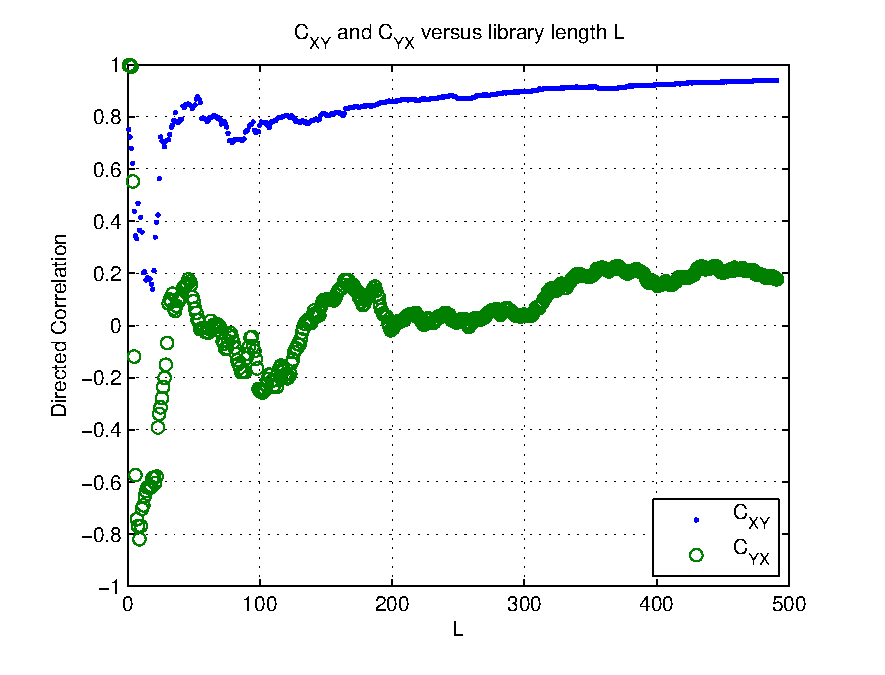
\includegraphics[scale=0.55]{CxyCyxVL.eps}
\caption{$\left(r_x,r_y,\beta_{xy},\beta_{yx},X(t_0),Y(t_0)\right) = \left(3.8,3.5,0.01,0.2,0.4,0.2\right)$ with $\tau=1$ and $E=2$.}
\end{figure}
Both directed correlations appear to converge to some nominal value and $C_{YX}<C_{XY}$ over most of the range (as expected).  But, notice that the small library length behaviour does not appear to follow expectations (i.e.\ $C_{YX}>C_{XY}$ for small $L$).

If instead the library length is fixed and the embedding dimension is varied, then the behaviour of the directed correlation changes dramatically.  Figure \ref{fig:CxyCyxVE} shows $C_{XY}$ and $C_{YX}$ calculated using all of the parameter values from above (and with $L=100$) but with the embedding dimension $E$ ranging from 2 to 50.  There are points over the embedding range when $C_{YX}<C_{XY}$ but there are also points where $C_{YX}>C_{XY}$, which is difficult to interpret with the given parameter set.  The dependence on the embedding dimension is concerning because it implies that incorrect conclusions can be drawn about natural data sets (i.e.\ time series where the theoretical dynamics are not known) regarding which directed correlation is dominate (i.e.\ which time series is the dominate ``driver'').  Similar issues arise when plotting the directed correlation over a range for the time step $\tau$ from 1 to 25 (see Figure \ref{fig:CxyCyxVtau}).  
\begin{figure}[h!t]
\centering
\begin{subfigure}[b]{0.4\textwidth}
\label{fig:CxyCyxVE}
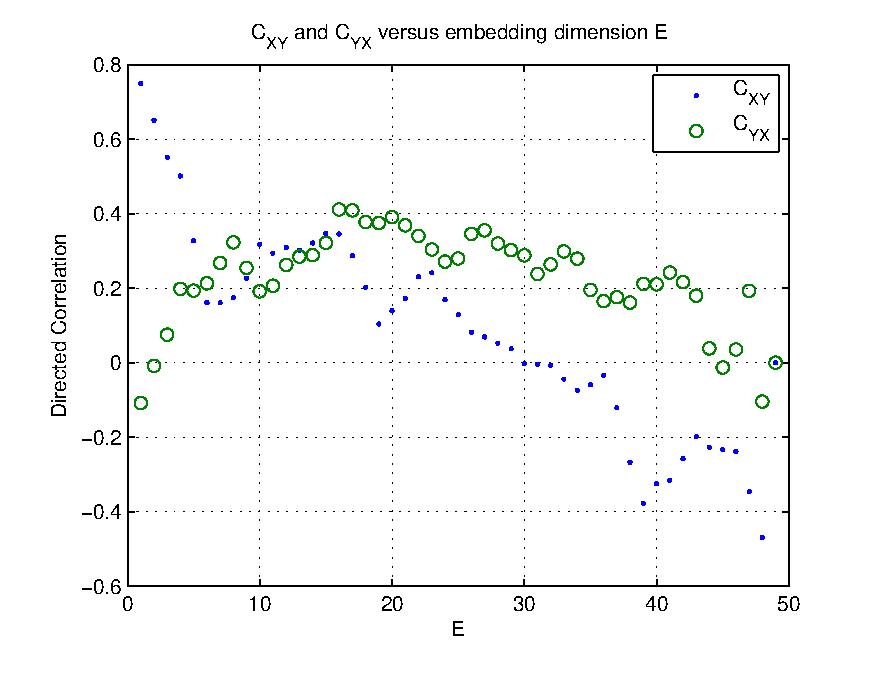
\includegraphics[scale=0.55]{CxyCyxVE.eps}
\caption{$\left(r_x,r_y,\beta_{xy},\beta_{yx},X(t_0),Y(t_0)\right) = \left(3.8,3.5,0.01,0.2,0.4,0.2\right)$ with $\tau=1$ and $L=100$.}
\end{subfigure}
\begin{subfigure}[b]{0.4\textwidth}
\label{fig:CxyCyxVtau}
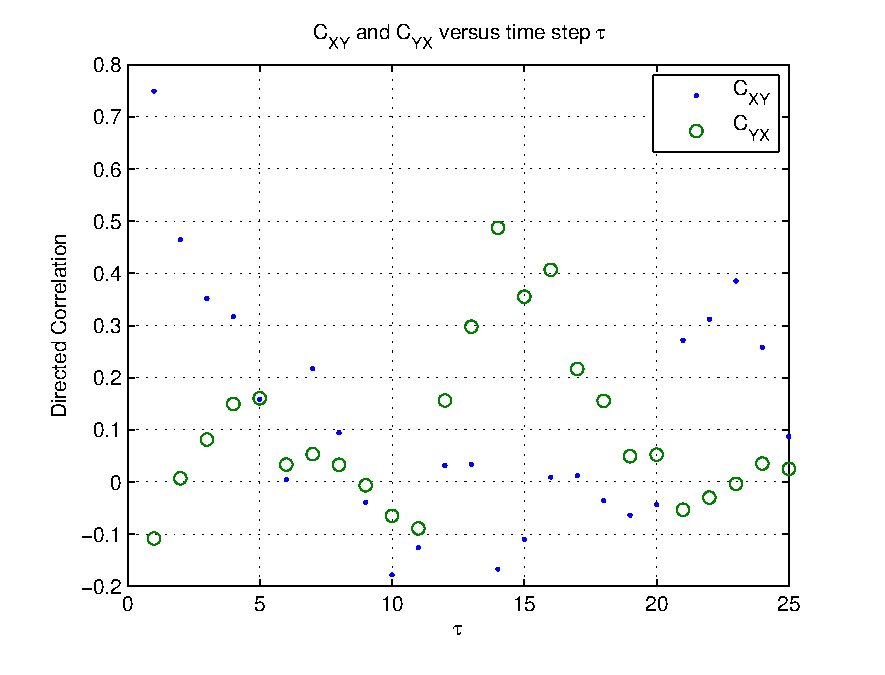
\includegraphics[scale=0.55]{CxyCyxVtau.eps}
\caption{$\left(r_x,r_y,\beta_{xy},\beta_{yx},X(t_0),Y(t_0)\right) = \left(3.8,3.5,0.01,0.2,0.4,0.2\right)$ with $E=2$ and $L=100$.}
\end{subfigure}
\caption{}
\end{figure}

The directed correlation acts as expected for $L=100$, $E=2$, and $\tau=1$.  These values can be used (along with $r_x$ and $r_y$) to see how the directed correlation behaves over a range of $\beta_{yx}$ given $\beta_{xy}=0.5$.  Figure \ref{fig:CxyCyxVByx_raw} shows $C_{YX}$ and $C_{XY}$ plotted over the range $\beta_{yx}\in[0.01,1.0]$ (with $\beta_{xy}=0.5$), and Figure \ref{fig:CxyCyxVByx_diff} shows the difference $\Delta = (C_{XY}-C_{YX})$ over the same range.
\begin{figure}[h!t]
\centering
\begin{subfigure}[b]{0.4\textwidth}
\label{fig:CxyCyxVByx_raw}
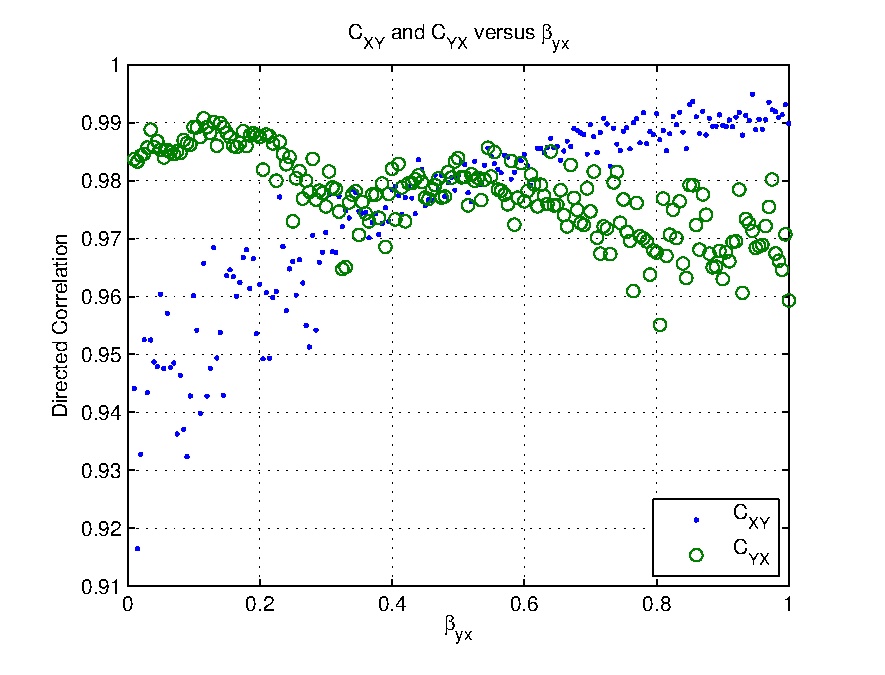
\includegraphics[scale=0.55]{CxyCyxVByx_raw.eps}
\caption{$\left(r_x,r_y,\beta_{xy},X(t_0),Y(t_0)\right) = \left(3.8,3.5,0.5,0.4,0.2\right)$ with $\left(E,L,\tau\right)=\left(2,500,1\right)$.}
\end{subfigure}
\begin{subfigure}[b]{0.4\textwidth}
\label{fig:CxyCyxVByx_diff}
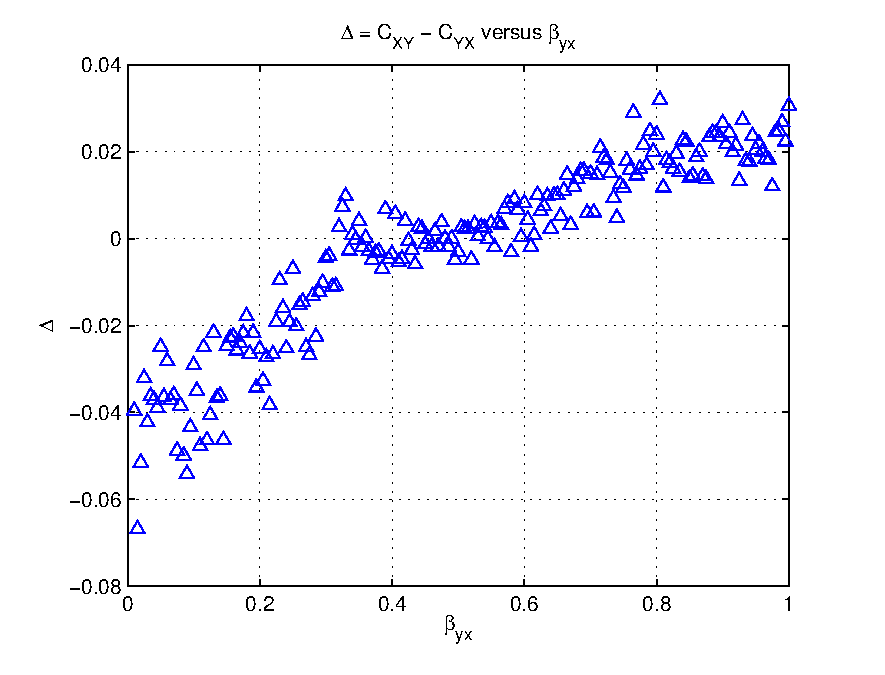
\includegraphics[scale=0.55]{CxyCyxVByx_diff.eps}
\caption{$\left(r_x,r_y,\beta_{xy},X(t_0),Y(t_0)\right) = \left(3.8,3.5,0.5,0.4,0.2\right)$ with $\left(E,L,\tau\right)=\left(2,500,1\right)$.}
\end{subfigure}
\caption{}
\end{figure}
Notice that $\Delta$ is an increasing function of $\beta_{yx}$ that crosses zero around $\beta_{yx}=0.5$, as expected given the discussion of the CCM algorithm in the beginning sections.  Figure \ref{fig:CxyCyxVByxBxy_diff} is a plot of $\Delta$ of ranges for both coupling constants, i.e.\ $\beta_{xy}\in[0.01,1.0]$ and $\beta_{yx}\in[0.01,1.0]$.
\begin{figure}[h!t]
\centering
\label{fig:CxyCyxVByxBxy_diff}
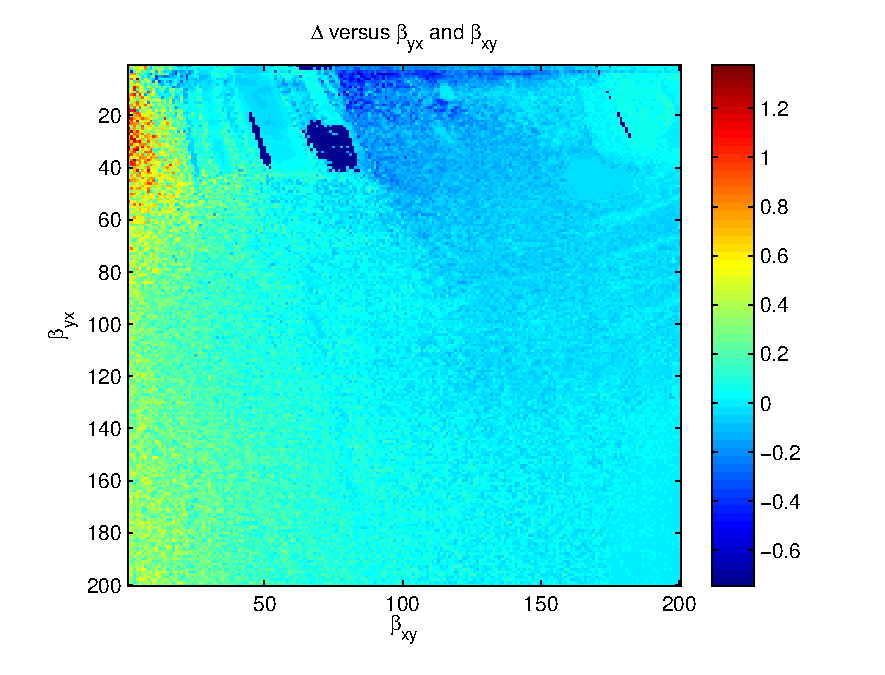
\includegraphics[scale=0.55]{CxyCyxVByxBxy_diff.eps}
\caption{$\left(r_x,r_y,X(t_0),Y(t_0)\right) = \left(3.8,3.5,0.2,0.4,0.2\right)$ with $\left(E,L,\tau\right)=\left(2,100,1\right)$.}
\end{figure}
Following the intuitive expectation, $\beta_{xy}>\beta_{yx}\Rightarrow \Delta<0$ and $\beta_{xy}<\beta_{yx}\Rightarrow \Delta>0$.

Notice, $\Delta$ is not symmetric about zero for the pair $(\beta_{xy},\beta_{yx})$; i.e.\
$$
\left(\beta_{xy},\beta_{yx}\right) = \left(0.5,0.01\right) \Rightarrow \Delta \approx -0.27\;\;,
$$
but
$$
\left(\beta_{xy},\beta_{yx}\right) = \left(0.01,0.5\right) \Rightarrow \Delta \approx 0.42
$$
which is positive but not 0.27.  The difference $\Delta$ is symmetric about zero given the entire parameter set for each time series, i.e.\
$$
\left(r_x,r_y,\beta_{xy},\beta_{yx},X(t_0),Y(t_0)\right) = \left(3.8,3.5,0.5,0.01,0.4,0.2\right) \Rightarrow \Delta \approx -0.27
$$
and
$$
\left(r_x,r_y,\beta_{xy},\beta_{yx},X(t_0),Y(t_0)\right) = \left(3.5,3.8,0.01,0.5,0.2,0.4\right) \Rightarrow \Delta \approx 0.27\;\;.
$$

Given the results of this section, the CCM algorithm does provide a kind of coarse grained quantification of the idea of ``driving'' between two time series.  More specifically, the sign of $\Delta$ provides information about the relative strength of dependencies between two time series.

\section{Embedding Dimension and Lag Time Step}
The embedding dimension ($E$) dependence of the CCM algorithm in the above examples implies a strong need to understand that dependence in terms of the time series used to create the shadow manifold.  It would be difficult to justify any results derived from the use of the CCM method on empirical data (e.g.\ the solar data) without such an understanding.  The ideal solution would be the development of simple statistical procedures (e.g.\ through the use of autocorrelations, entropies, etc$.$) to find the ``correct'' embedding dimension $E_X$ given a times series $X$.

Consider the Sugihara example system with $\left(r_x,r_y,\beta_{xy},\beta_{yx},X(t_0),Y(t_0)\right) = \left(3.8,3.5,0.01,0.2,0.4,0.2\right)$.  Define the $l$-lagged autocorrelation $A_l^X$ of $X(t)$ as $A_l^X=\rho_{X(t),X(t-l)}$ given $t\in(l,L]$ where $L$ is the library length.  For this example system, both $|A_l^X|$ and $|A_l^Y|$ can be plotted as a function of $l$.  See Figure \ref{fig:autocorrSug}.
\begin{figure}[h!t]
\centering
\label{fig:autocorrSug}
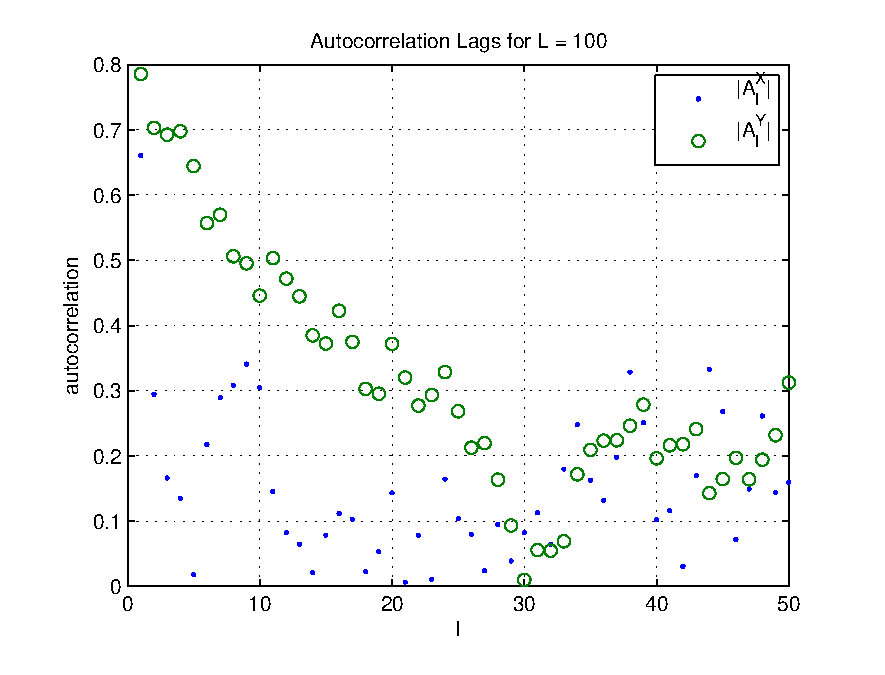
\includegraphics[scale=0.55]{autocorrSug.eps}
\caption{$\left(r_x,r_y,\beta_{xy},\beta_{yx},X(t_0),Y(t_0)\right) = \left(3.8,3.5,0.01,0.2,0.4,0.2\right)$.}
\end{figure}
The max and min of $|A_l^X|$ occur at $l=1$ and $l=21$, respectively, and the  max and min of $|A_l^Y|$ occur at $l=1$ and $l=30$.  Define $\Delta=C_{XY}-C_{YX}$.  Given the parameters of this example system, it is expected that $\Delta>0$ (because ``intuitively'', the parameter set seems to imply $X\Rightarrow Y$ for this example).  The embedding dimension dependence of $\Delta$ can be plotted to reiterate the conclusions of the previous section.  See Figure \ref{fig:SugDeltavE}.
\begin{figure}[h!t]
\centering
\begin{subfigure}[b]{0.4\textwidth}
\label{fig:SugDeltavE}
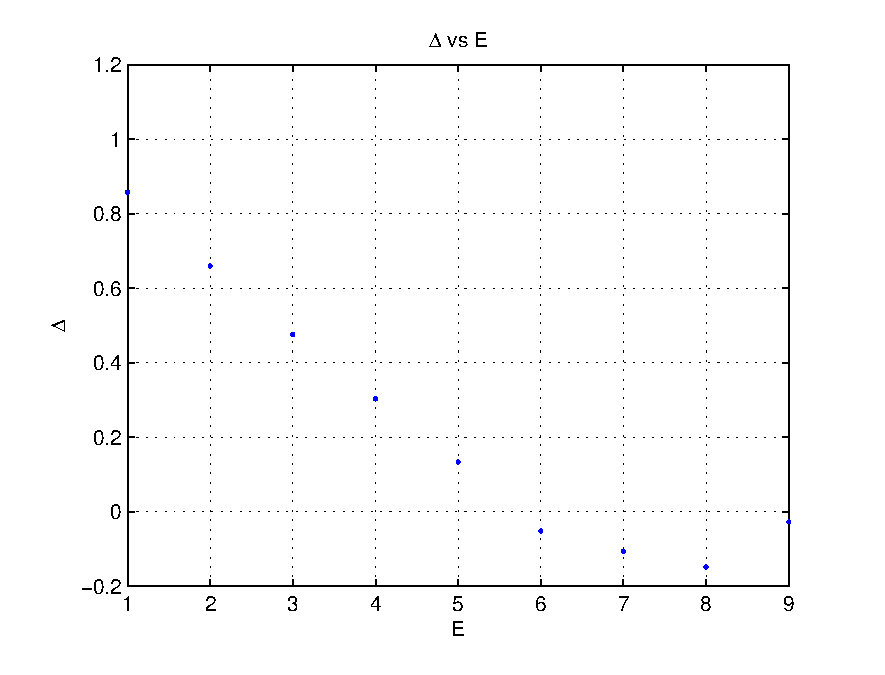
\includegraphics[scale=0.55]{SugDeltavE.eps}
\caption{$\left(r_x,r_y,\beta_{xy},\beta_{yx},X(t_0),Y(t_0)\right) = \left(3.8,3.5,0.01,0.2,0.4,0.2\right)$ and $\left(L,\tau\right) = \left(100,1\right)$.}
\end{subfigure}
\begin{subfigure}[b]{0.4\textwidth}
\label{fig:SugDeltavEandL}
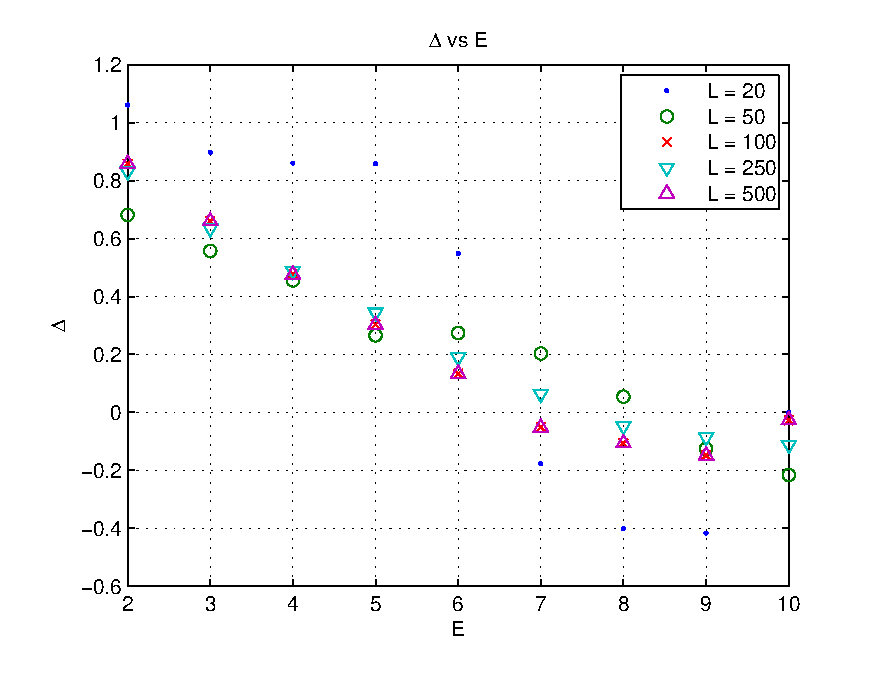
\includegraphics[scale=0.55]{SugDeltavEandL.eps}
\caption{$\left(r_x,r_y,\beta_{xy},\beta_{yx},X(t_0),Y(t_0)\right) = \left(3.8,3.5,0.01,0.2,0.4,0.2\right)$ and $ \tau = 1$.}
\end{subfigure}
\caption{}
\end{figure}
Notice $\Delta = \max_E \Delta$ for $E=2$ which corresponds a autocorrelation lag $l=1$.  So, it appears that for this example system, the required embedding dimension $E$ to achieve $\Delta=\max_E \Delta$ could be found by determining $l$ such that $|A_l^X|=\max_l |A_l^X|$ and $|A_l^Y|=\max_l |A_l^Y|$.  However, it can be seen from the plot that $E\in [2,5]\rightarrow \Delta>0$ and $E\in [6,10]\rightarrow \Delta<0$.  This change in sign of $\Delta$ does not appear to correlate with the autocorrelation lags in a straightforward way akin to the above relationship between $l$ and $\max_E \Delta$.  The lack of correlation between $l$ and the positivity of $\Delta$ may indicate the the relationship between $l$ and $\max_E \Delta$ is coincidental or a specific property of this example system.  Also notice the value of $E$ for which $\Delta$ changes signs depends on the library length $L$ (although, for this example at least, the value of $E$ such that $\Delta = \max_E \Delta$ seems to be independent of $L$).  See Figure \ref{fig:SugDeltavEandL} to see the data that leads to this observation.  Before these ideas are explored with other example systems, consider the question of why $E$ is the same for both shadow manifolds.

There does not seem to be any {\em a priori} reason that $E$ needs to be the same for both shadow manifolds used to calculate $\Delta$.  Figure \ref{fig:SugExVaryE} shows $\Delta$ as a function of the embedding dimension used to create the $X$ shadow manifold, $E_X$, and the embedding dimension used to create the $Y$ shadow manifold, $E_Y$.  
\begin{figure}[h!t]
\centering
\label{fig:SugExVaryE}
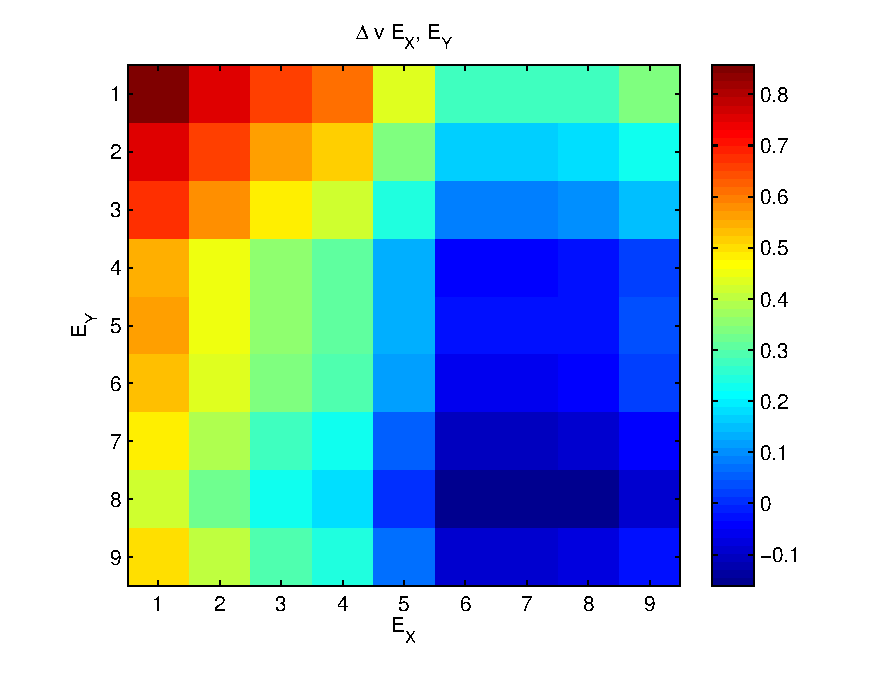
\includegraphics[scale=0.55]{SugExVaryE.eps}
\caption{$\left(r_x,r_y,\beta_{xy},\beta_{yx},X(t_0),Y(t_0)\right) = \left(3.8,3.5,0.01,0.2,0.4,0.2\right)$ and $\left(L,\tau\right) = \left(100,1\right)$.}
\end{figure}
Notice that $E_X \in [2,4]\rightarrow \Delta>0\;\forall E_Y\in[2,10]$ and $E_Y \in[2,6]\rightarrow \Delta>0\;\forall E_X\in[2,10]$.  So, at least for this example system and embedding dimensions $\in[2,10]$, achieving $\Delta>0$ is not necessarily dependent on both $E_X$ and $E_Y$.  

Consider the Sugihara example system with $\left(r_x,r_y,\beta_{xy},\beta_{yx},X(t_0),Y(t_0)\right) = \left(3.1,3.9,0.2,0.002,0.4,0.2\right)$.  This parameter set leads to the expectation of $\Delta<0$ and, indeed, $\Delta<0$ if $(L,\tau)=(100,1)$ with $E_X,E_Y\in[2,3]$.  See Figure \ref{fig:SugEx2VaryE}.
\begin{figure}[h!t]
\centering
\begin{subfigure}[b]{0.4\textwidth}
\label{fig:SugEx2VaryE}
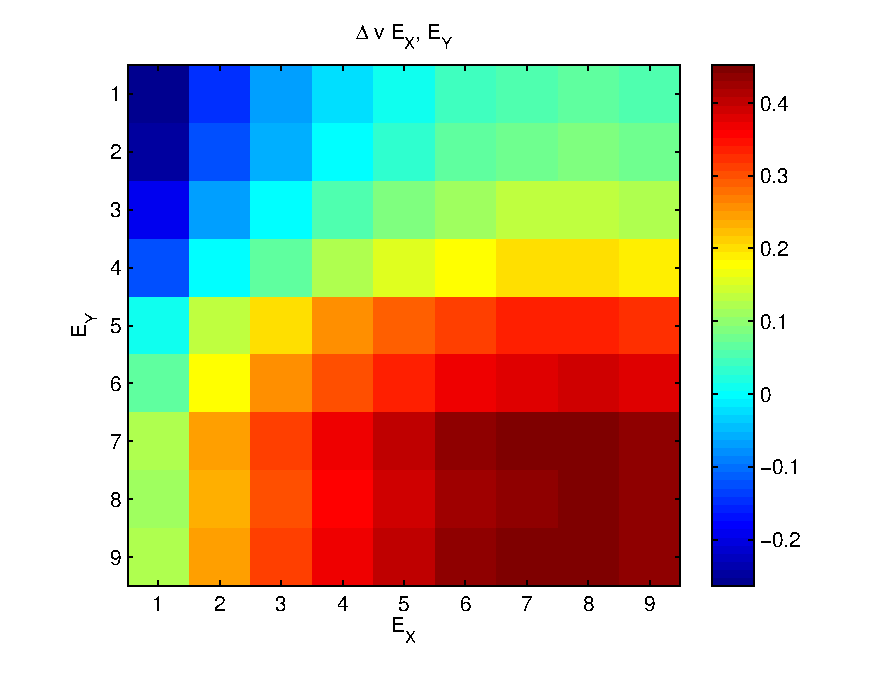
\includegraphics[scale=0.55]{SugEx2VaryE.eps}
\caption{$\left(r_x,r_y,\beta_{xy},\beta_{yx},X(t_0),Y(t_0)\right) = \left(3.1,3.9,0.2,0.002,0.4,0.2\right)$ and $\left(L,\tau\right) = \left(100,1\right)$.}
\end{subfigure}
\begin{subfigure}[b]{0.4\textwidth}
\label{fig:SugEx2VaryEauto}
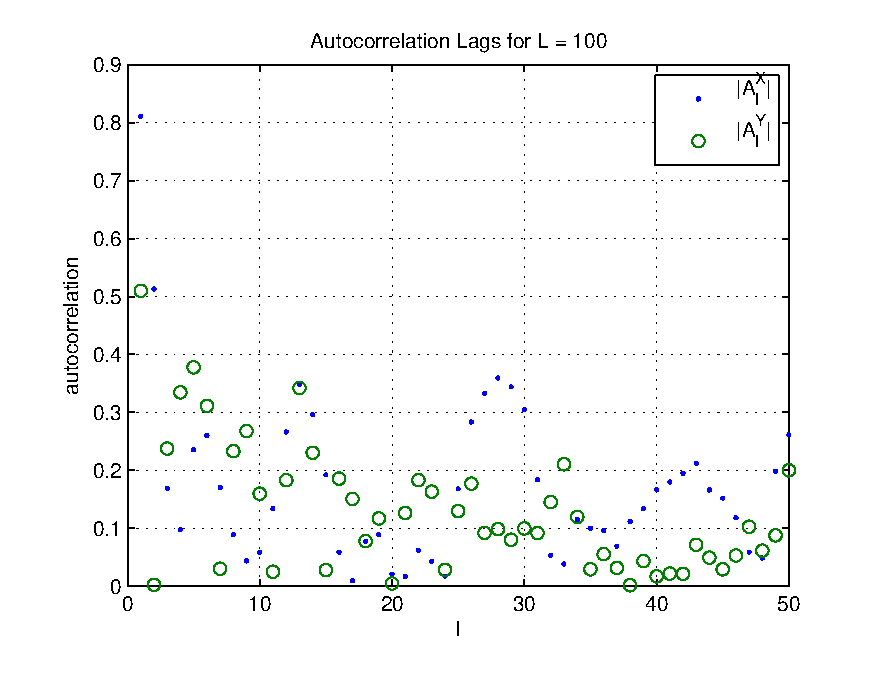
\includegraphics[scale=0.55]{SugEx2VaryEauto.eps}
\caption{$\left(r_x,r_y,\beta_{xy},\beta_{yx},X(t_0),Y(t_0)\right) = \left(3.1,3.9,0.2,0.002,0.4,0.2\right)$ and $\left(L,\tau\right) = \left(100,1\right)$.}
\end{subfigure}
\caption{}
\end{figure}
Plotting $|A_l^X|$ and $|A_l^Y|$ for this example system (see Figure \ref{fig:SugEx2VaryEauto}) reveals $|A_l^X|=\max_l |A_l^X|$ and $|A_l^Y|=\max_l |A_l^Y|$ for $l=1$, just as in the example of the previous paragraphs.  So, the above method to determine the ``correct'' embedding dimension from the data using autocorrelation lags seems to provide answers that agree with intuition in at least two examples.  Although it should be noted that in the second example, preserving the intuitive conclusion (i.e. $\Delta<0$) cannot be achieved with $E_X=2$ with any $E_Y\in[2,10]$ or $E_Y$ with any $E_X\in[2,10]$.  In constraint to the first example, it is possible in the second example to achieve $\Delta>0$ with $E_{X(Y)}=2$ and $E_{Y(X)}\in[6,10]$.

The shadow manifold is used to estimate the time series of interest, so it seems reasonable that the embedding dimension of the shadow manifold should be related to the autocorrelation lag of the time series of interest rather than the times series used to create the shadow manifold.  Notice that this approach would not change the relationship between $l$ and $\max_E \Delta$ discussed in the previous paragraph.

Using the autocorrelation method discussed above may provided embedding dimensions that agree with intuition, but the method does not explain the apparent dependence of the CCM on embedding dimension.  As an attempt o understand this dependence consider the following algorithm (``NN1''): 
\begin{enumerate}
\item Embed $X$ in a manifold with dimension $E$.
\item Record the time step locations $\tilde{t}^E_i$ (in the original $X$) and weights $w^E_i$ of the $N=E+1$ dimensional point $X(t)$ 
\item Repeat steps 1 and 2 for $E=E+1$.
\item Stop when $\{\tilde{t}_i^E\} \neq \{\tilde{t}_i^{E-1}\}$; i.e.\ stop when the set of time step locations in the $N$-dimensional point given $E$ is not the same as the set of time step locations in the $N$-dimensional point given $E-1$.  (Notice that the algortihm completely ignores $\{w_i^E\}$.)
\item Record $E$ (i.e.\ the embedding dimension for which the above iteration is halted) as $E^H_t$.
\item Repeat steps 1-4 for $t=t+1$ for all $t\le T$ where $T$ is dependent on the library length $L$ of $X$ .
\item Find the mode of $\{E_t^H\}$.
\end{enumerate}
Also consider the following, very similar, algorithm (``NN2''):
\begin{enumerate}
\item Embed $X$ in a manifold with dimension $E$.
\item Record the time step locations $\tilde{t}^E_i$ (in the original $X$) and weights $w^E_i$ of the $N=E+1$ dimensional point $X(t)$ 
\item Repeat steps 1 and 2 for $E=E+1$.
\item Stop when $\exists w^E_i < \delta$; i.e.\ stop when one of the weights $N$-dimensional point drops below some cutoff value $\delta$.  (Notice that the algortihm completely ignores $\{t_i^E\}$.)
\item Record $E$ (i.e.\ the embedding dimension for which the above iteration is halted) as $E^H_t$.
\item Repeat steps 1-4 for $t=t+1$ for all $t\le T$ where $T$ is dependent on the library length $L$ of $X$ .
\item Find the mode of $\{E_t^H\}$.
\end{enumerate}
The second algorithm (NN2) requires the selection of some $\delta$ and both algorithms require determining $T$.  Consider the Sugihara example with $\left(r_x,r_y,\beta_{xy},\beta_{yx},X(t_0),Y(t_0)\right) = \left(3.8,3.5,0.01,0.2,0.4,0.2\right)$ and $\left(L,\tau\right) = \left(100,1\right)$.  Applying NN1 to $X$ yields 7 for $T\in[1,50]$.  Applying NN2 to $X$ with $T=10$ yields 2 for $\delta=0.05$ and $\delta=0.01$.  The addition of the free parameter $\delta$ makes NN2 a little less convincing than NN1 (e.g.\ how is a particular choice for $\delta$ justified?).  The behaviour of NN2 on $X$ for $T\in[1,50]$ and $\delta\in[10^{-5},10^{-2}]$ (in steps of ??) can be seen in \ref{fig:SugExNN1vTvd}.

It might be assumed that the dependence of $\Delta$ on $E$ implies a similar dependence of $\Delta$ on the lagged time step $\tau$ because of (co-dependent?) roles $E$ and $\tau$ play in the construction of the shadow manifold.  To explore these idea, introduce $\tau_X$ and $\tau_Y$ in analogy to $E_X$ and $E_Y$.  Figures \ref{fig:SugExvTauXY} and \ref{fig:SugExvTauXvTauY} show $\Delta$ does have a dependency on $\tau_{X (Y)}$ and, like $E_{X(Y)}$, leads to ``unintuitive'' results for large $\tau$.
\begin{figure}[h!t]
\centering
\begin{subfigure}[b]{0.4\textwidth}
\label{fig:SugExvTauXY}
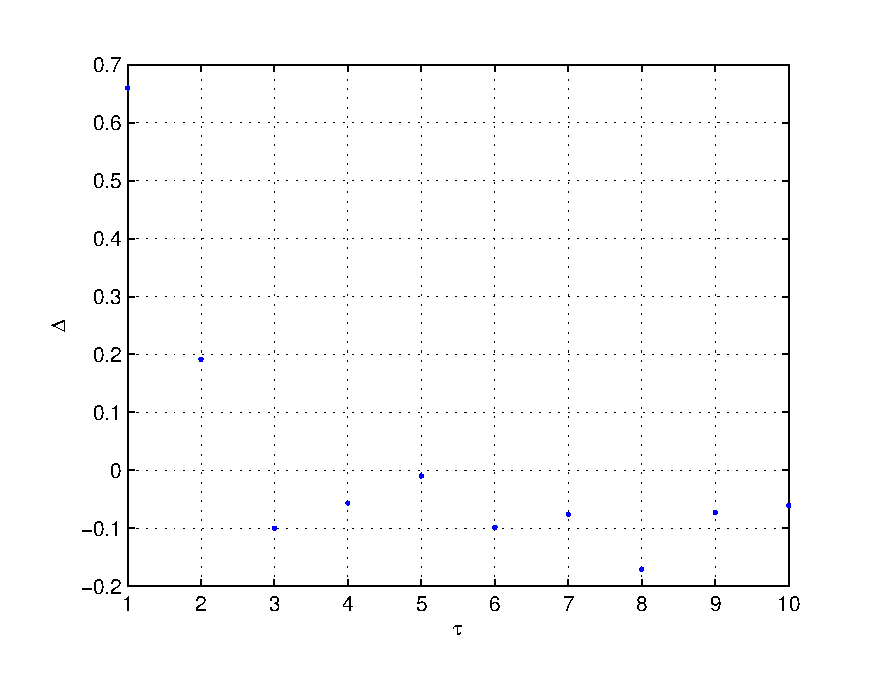
\includegraphics[scale=0.55]{SugExvTauXY.eps}
\caption{ $\left(r_x,r_y,\beta_{xy},\beta_{yx},X(t_0),Y(t_0)\right) = \left(3.8,3.5,0.01,0.2,0.4,0.2\right)$ and $\left(L,E\right) = \left(100,3\right)$ with $\tau_X=\tau_Y$.}
\end{subfigure}
\begin{subfigure}[b]{0.4\textwidth}
\label{fig:SugExvTauXvTauY}
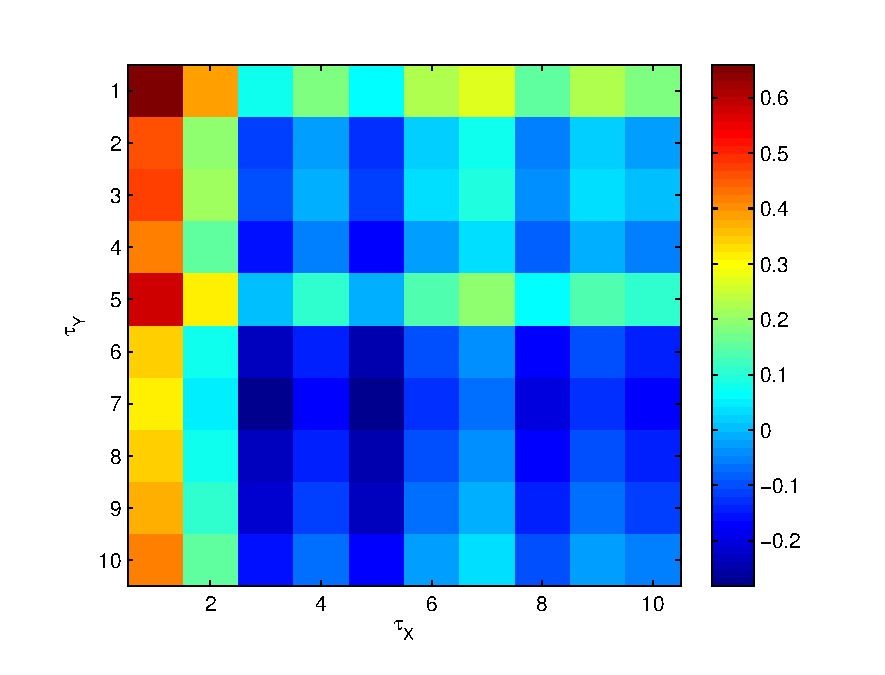
\includegraphics[scale=0.55]{SugExvTauXvTauY.eps}
\caption{ $\left(r_x,r_y,\beta_{xy},\beta_{yx},X(t_0),Y(t_0)\right) = \left(3.8,3.5,0.01,0.2,0.4,0.2\right)$ and $\left(L,E\right) = \left(100,3\right)$.}
\end{subfigure}
\caption{}
\end{figure}
To reinforce the idea, Figures \ref{fig:SugEx2vTauXY} and \ref{fig:SugEx2vTauXvTauY} show similar results for the Sugihara system with the coefficients used to produce Figure {fig:SugEx2VaryE}.
\begin{figure}[h!t]
\centering
\begin{subfigure}[b]{0.4\textwidth}
\label{fig:SugEx2vTauXY}
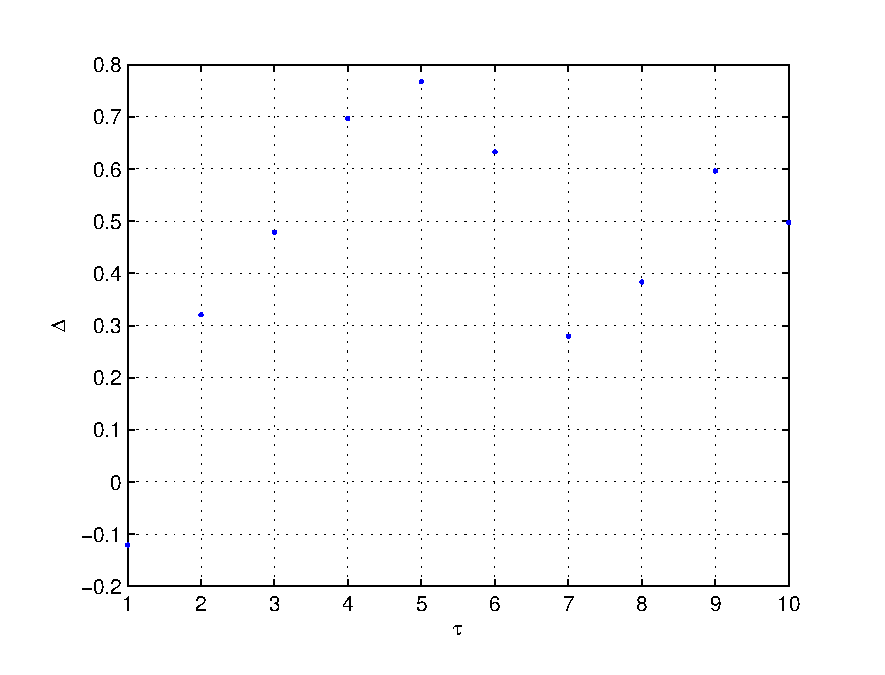
\includegraphics[scale=0.55]{SugEx2vTauXY.eps}
\caption{ $\left(r_x,r_y,\beta_{xy},\beta_{yx},X(t_0),Y(t_0)\right) = \left(3.1,3.9,0.2,0.002,0.4,0.2\right)$ and $\left(L,E\right) = \left(100,3\right)$. with $\tau_X=\tau_Y$.}
\end{subfigure}
\begin{subfigure}[b]{0.4\textwidth}
\label{fig:SugEx2vTauXvTauY}
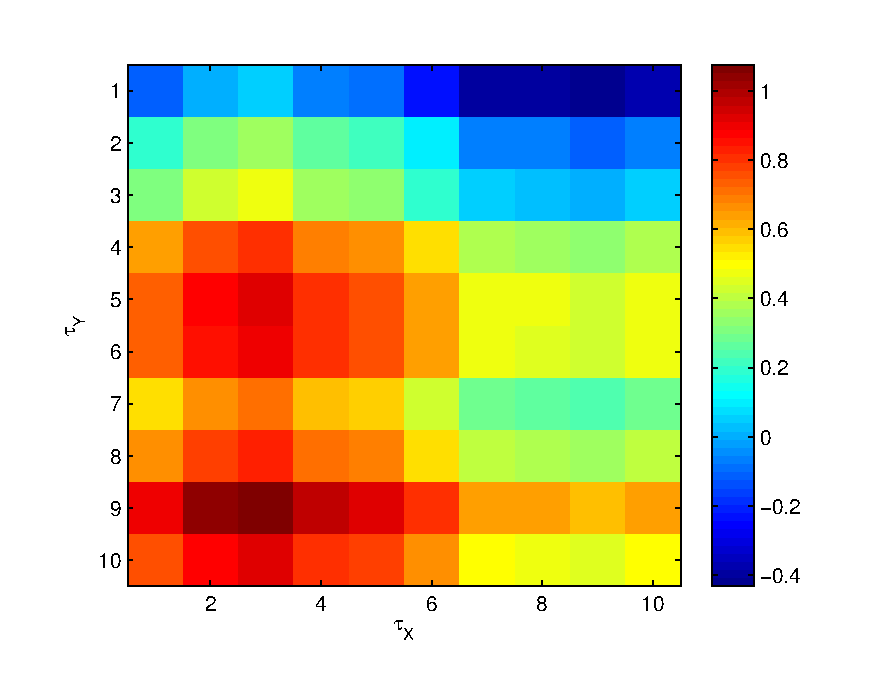
\includegraphics[scale=0.55]{SugEx2vTauXvTauY.eps}
\caption{ $\left(r_x,r_y,\beta_{xy},\beta_{yx},X(t_0),Y(t_0)\right) = \left(3.1,3.9,0.2,0.002,0.4,0.2\right)$ and $\left(L,E\right) = \left(100,3\right)$.}
\end{subfigure}
\caption{}
\end{figure}
Notice that both examples lead to unintuitive results much quicker as $\tau_{X(Y)}$ is increased then when $E_{X(Y)}$ was increased.  This apparent larger sensitivity of the CCM algorithm on $\tau$ than $E$ implies that care most be taken to carefully choose both.  The autocorrelation method proposed above to find $E$ also works to find the lagged time step $\tau$ with the largest intuitive results; i.e.\ $|A_l^X|=\max_l |A_l^X|$ and $|A_l^Y|=\max_l |A_l^Y|$ for $l=1$ (for both examples discussed in this paragraph) and $\Delta = \max_\tau \Delta$ for $\tau=1$ with $\tau_{X(Y)}=1$ (again, for both examples).  Hence, the autocorrelation method may be a good option for determining $\tau_{X(Y)}$.

As expected, there is also a co-dependence of $\Delta$ on $E$ and $\tau$ if both are changed simultaneously, as seen in Figures \ref{fig:SugEx2vEdimvTau} and \ref{fig:SugEx2vEdimvTau} for both examples discussed in the previous paragraphs.
\begin{figure}[h!t]
\centering
\begin{subfigure}[b]{0.4\textwidth}
\label{fig:SugEx2vEdimvTau}
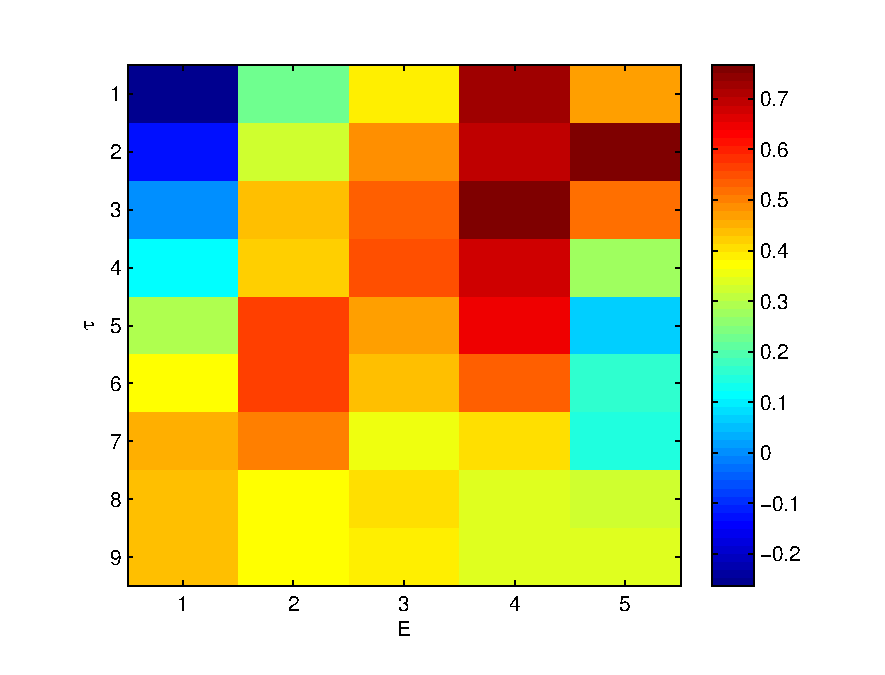
\includegraphics[scale=0.55]{SugEx2vEdimvTau.eps}
\caption{ $\left(r_x,r_y,\beta_{xy},\beta_{yx},X(t_0),Y(t_0)\right) = \left(3.1,3.9,0.2,0.002,0.4,0.2\right)$ and $\left(L\right) = \left(100\right)$. with $\tau_X=\tau_Y$ and $E_X=E_Y$.}
\end{subfigure}
\begin{subfigure}[b]{0.4\textwidth}
\label{fig:SugEx1vEdimvTau}
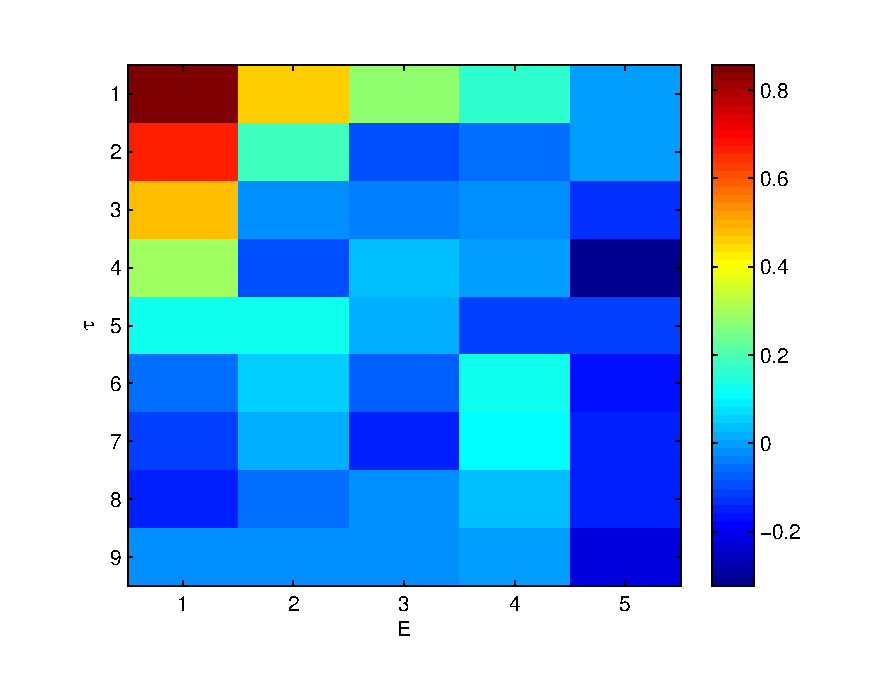
\includegraphics[scale=0.55]{SugEx1vEdimvTau.eps}
\caption{ $\left(r_x,r_y,\beta_{xy},\beta_{yx},X(t_0),Y(t_0)\right) = \left(3.8,3.5,0.01,0.2,0.4,0.2\right)$ and $\left(L\right) = \left(100\right)$ with $\tau_X=\tau_Y$ and $E_X=E_Y$.}
\end{subfigure}
\caption{}
\end{figure}
This co-dependence complicates the use of an algorithm like NN1 or NN2 to determine $E$ (or $\tau$) because of the use of the points in the shadow manifold (which depends on both parameter, rather than just the one parameter being iterated).  This shortcoming can be overcoming by extending NN1 (or NN2) to included iterations over both parameters (e.g.\ called NN1$_{ex}$ or NN2$_{ex}$ to effectively search the entire 2D parameter space of $(E,\tau)$ and applying exactly the same logic as used in the original NN1 (or NN2) algorithm.  Unfortunately, the changes necessary to NN1(2) to create NN1(2)$_{ex}$ introduce a computational load that would make the algorithms difficult to apply to large datasets (like the solar data).  As such, the autocorrelation method (which is independent of the shadow manifold) can be used to set the lagged time step $\tau$ and then NN1 (or NN2) can be used to determine $E$.  This two step process to determine ``reasonable'' parameters for the CCM algorithm will be explored outside of the Sugihara example in the next section.

As a final note, notice that the ``intuitive/unintuitive result'' cutoff (let's call this $c_u$ so I can stop writing ``intuitive'') depends not only on $E$ and $\tau$ (as was shown above) but also on the parameters of the system itself.  This complicated behaviour of $c_u$ makes it frustrating (perhaps impossible?) to understand it in terms of the CCM algorithm parameters alone.  As an illustration of this point, set $\left(r_x,r_y,\beta_{xy},X(t_0),Y(t_0)\right) = \left(3.8,3.5,0.01,0.4,0.2\right)$ and $\left(L,\tau\right) = \left(100,1\right)$ where $\tau_X=\tau_Y=\tau$.  Plotting $\Delta$ versus $E=E_X=E_Y$ for different values of $\beta_{yx}$ reveals that $c_u$ varies with $\beta_{yx}$ (see Figure \ref{fig:SugExvEdimvByx}).
\begin{figure}[h!t]
\centering
\label{fig:SugExvEdimvByx}
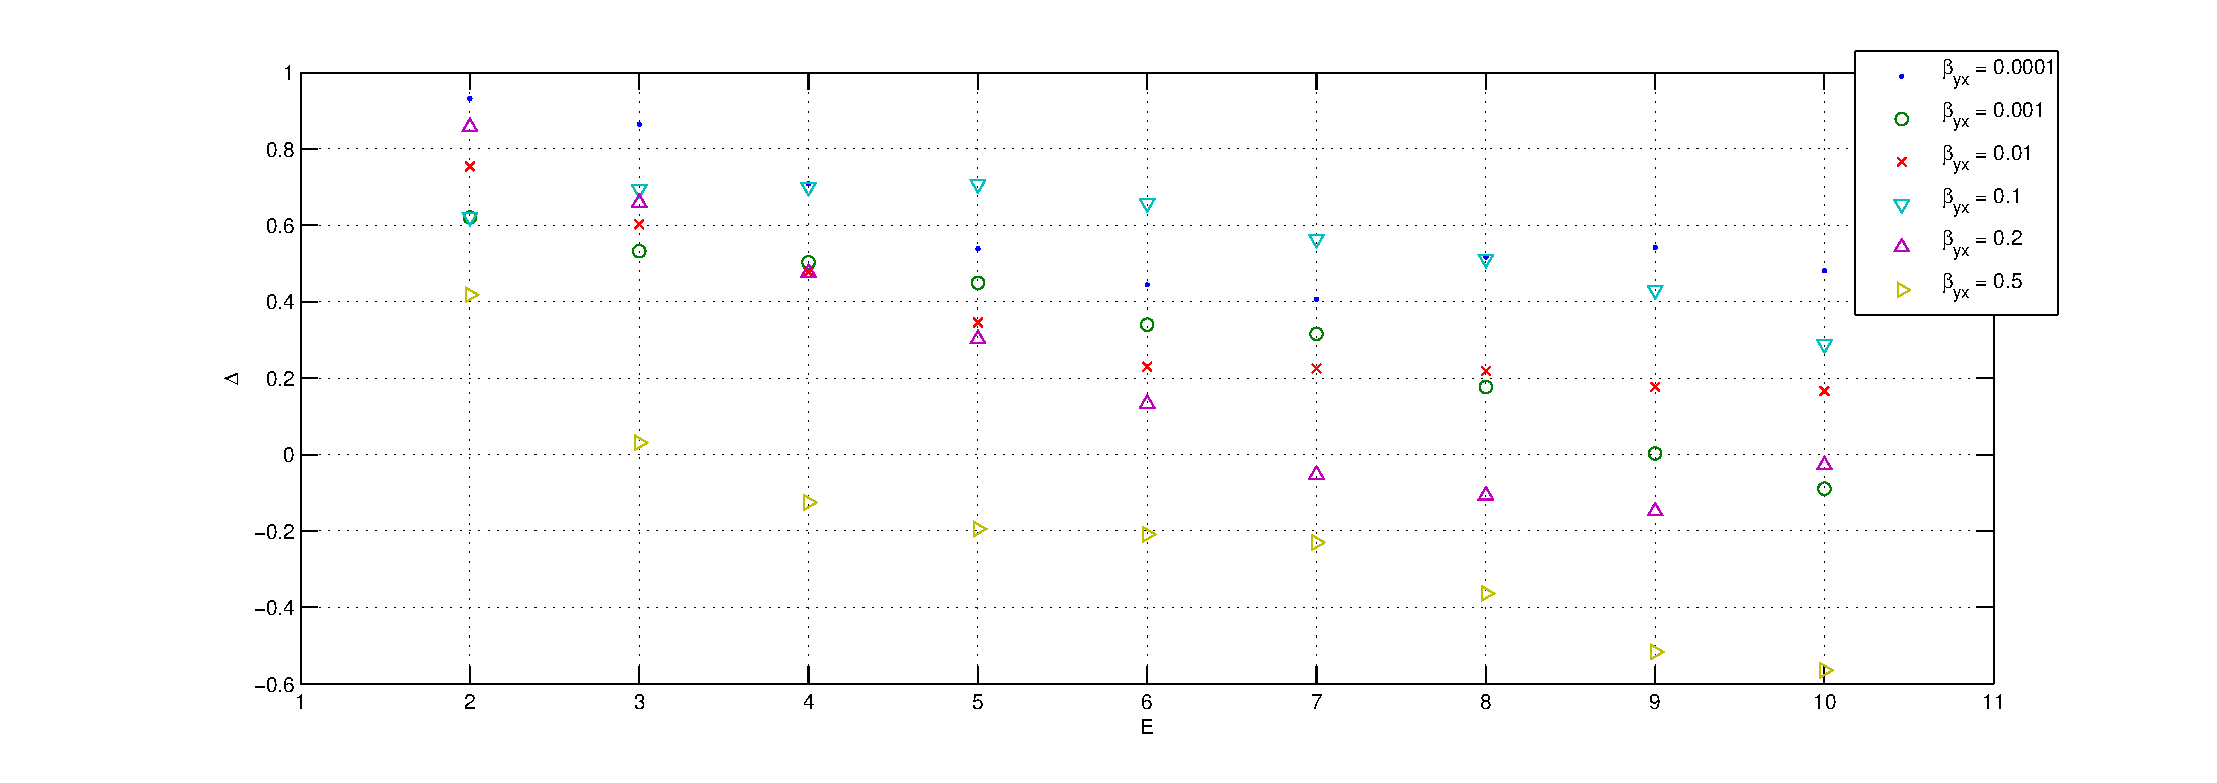
\includegraphics[scale=0.55]{SugExvEdimvByx.eps}
\caption{$\left(r_x,r_y,\beta_{xy},X(t_0),Y(t_0)\right) = \left(3.8,3.5,0.01,0.4,0.2\right)$ and $\left(L,\tau\right) = \left(100,1\right)$ where $\tau_X=\tau_Y=\tau$ and $E_X=E_Y$.}
\end{figure}
Given the dynamics of the Sugihara example it would seem, if everything else is kept constant, that $X$ is a stronger driver of $Y$ as $\beta_{yx}$ increases.  Unfortunately, such ``intuition'' is not seen in the resulting figure.  Notice $\beta_{yx} = 10^{-4}$ (which obeys $\beta_{yx} < \beta_{xy}$) leads to no $c_u$ with the plotted range of $E\in[2,10]$.  The other plotted values of $\beta_{yx}$ show a wide variety of $c_u$ that have no obvious relationship to each other.  It is hard to have confidence in the application of the CCM method to measured data sets when this type of behaviour is so difficult to understand even in example systems.

\section{Sampling the Two Population Dynamics (Sugihara Example)}
The two-population dynamical system used Sugihara {\em et.\ al.\ },
\begin{eqnarray*}
X(t) &=& X(t-1)\left(r_x-r_x X(t-1)-\beta_{xy} Y(t-1)\right)\\
Y(t) &=& Y(t-1)\left(r_y-r_y Y(t-1)-\beta_{yx} X(t-1)\right)
\end{eqnarray*}
where $r_x,r_y,\beta_{xy},\beta_{yx}\in\mathbf{R}$, is very sensitive both the initial condition $X(t_0)$ and $Y(t_0)$ but also the dynamics parameters $r_x$, $r_y$, $\beta_{xy}$, and $\beta_{yx}$.  Consider the following table of values for $X$ and $Y$:
\begin{center}
\begin{table}[h!t]
\begin{tabular}{cccc}
          & $X(t) = -1$ & $X(t) = 0$ & $X(t) = 1$ \\
$Y(t) = -1$ & $(-2r_x-\beta_{xy},-2r_y-\beta_{yx})$ & $(0,-2r_y)$ & $(\beta_{xy},\beta_{yx}-2r_y)$\\
$Y(t) = 0$  & $(-2r_x,0)$ & $(0,0)$     & $(0,0)$\\
$Y(t) = 1$  & $(\beta_{xy}-2r_x,\beta_{yx})$ & $(0,0)$     & $(-\beta_{xy},-\beta_{yx})$\\
\end{tabular}
\caption{The entries are $(X(t+1),Y(t+1))$.}
\end{table}
\end{center}
The points $X(t) = 0$ and $Y(t) = 0$ are fixed points for this system.  The change in $X$ (or $Y$) can be derived as follows:
\begin{equation}
X(t) - X(t-1) = r_x\left(X(t-1)-\left(X(t-1)\right)^2-X(t-2)+\left(X(t-2)\right)^2\right) + \beta_{xy}\left(X(t-2)Y(t-2)-X(t-1)Y(t-1)\right)
\end{equation}
Let $\delta_t = X(t) - X(t-1)$.  The above equation can then be rewritten as
\begin{equation}
\delta_t = \delta_{t-1} r_x \left(1-X(t-1)-X(t-2)\right) + + \beta_{xy}\left(X(t-2)Y(t-2)-X(t-1)Y(t-1)\right)
\end{equation}
The parameters $r_x$ and $r_y$ can, as seen in the above equation, can lead to rapid growth of the time series to infinity (it is assumed that $\beta_{xy}$ and $\beta_{yx}$ are fixed).  The change between steps $t$ and $t-1$ depends on $r_x$ times the change between steps $t-1$ and $t-2$; i.e.\ a large $r_x$ can lead to a rapid growth in the change of $X$ between time steps.  As such, the parameters need to be carefully set to insure an oscillating system, which is our desire when testing the CCM algorithm.

All of the previous results using this Sugihara example used fixed values for $r_x$, $r_y$, $\beta_{yx}$, and $\beta_{xy}$ with fixed initial conditions $X(t_0)$ and $Y(t_0)$.  These values can be sampled (from some reasonable distribution) to investigate the ``robustness'' of the directed correlation concept.  More specifically, if the directed correlation is assumed to have a ``reasonable'' interpretation related to the coupling in the dynamics (i.e.\ $\beta_{yx}$ and $\beta_{xy}$), then varying the initial conditions and dynamics parameters (i.e.\ $r_x$ and $r_y$) should still lead to ``intuitive'' results.  

The initial conditions will be sampled from normal distributions with means $\mu_{x0}$ and $\mu_{y0}$ and variances $\sigma^2_{x0}$ and $\sigma^2_{y0}$.  Likewise, the dynamics parameters will be sampled from normal distributions with means $\mu_{rx}$ and $\mu_{ry}$ and variances $\sigma^2_{rx}$ and $\sigma^2_{ry}$.  The CCM algorithm parameters $E$ (embedding dimension) and $\tau$ (lag time step) will be set to 3 and 1, respectively, following the discussion of the previous section.  Of course, that still leaves the algorithm parameter of library length for this example (i.e.\ the time series is created computationally using the two-population dynamics model, so the library length is only limited by practical concerns of computational resources).  Figure \ref{fig:TwoPopDynvLL} reveals the same dependence on library length seen in the previous section with $\beta_{xy}=0.02$ and $\beta_{yx}=0.1$.
\begin{figure}[h!t]
\centering
\label{fig:TwoPopDynvLL}
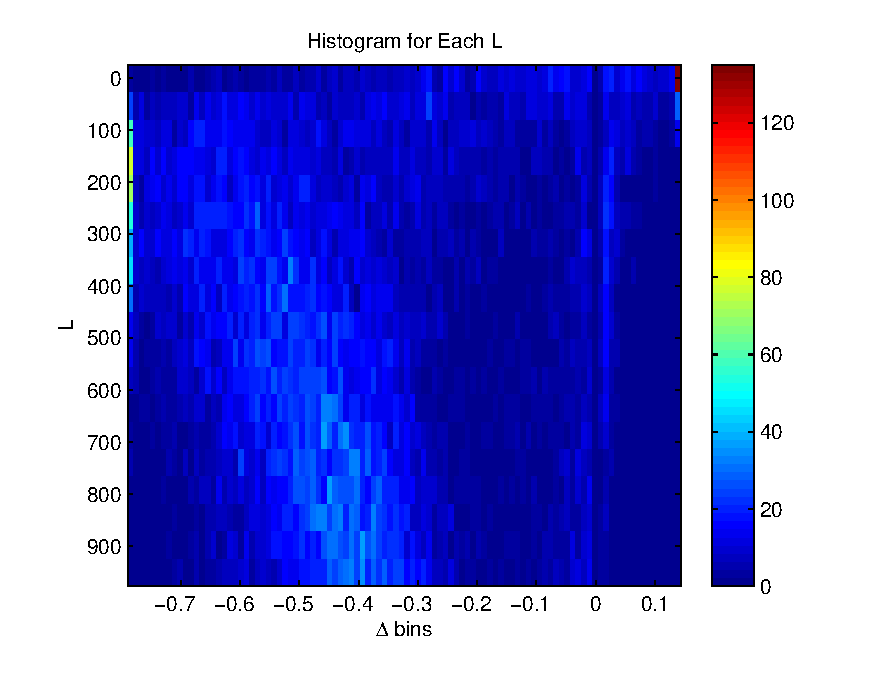
\includegraphics[scale=0.55]{TwoPopDynvLL.eps}
\caption{1000 samples with $\left(\mu_{rx},\mu_{ry},\sigma^2_{rx},\sigma^2_{ry},\mu_{x0},\mu_{y0},\sigma^2_{x0},\sigma^2_{y0}\right) = \left(3.8,3.5,0.1,0.1,0.4,0.2,0.3,0.3\right)$ and $\left(E,\tau\right)=\left(3,1\right)$ for $L=51, 101, 151, \ldots, 1000$ with ``zeroes removed'' (see text for a discussion of zero removal).}
\end{figure}

Notice that there are dynamic parameter combination that occur within this sample space (as defined in the previous paragraph) with non-negligible probability that cause the dynamical system to (rapidly) diverge (i.e.\ $X(t)\rightarrow \pm \infty$ and $Y(t)\rightarrow \pm \infty$ as $t\rightarrow\infty$) or reach a fixed point as described above.  For example, $\left(r_x,r_y,X(t_0),Y(t_0)\right) = \left(4.04,3.39,7.31x10^{-2},4.94x10^{-2}\right)$ and $\left(r_x,r_y,X(t_0),Y(t_0)\right) = \left(3.85,3.49,1.00,4.56x10^{-1}\right)$ cause the system to diverge and occurred within a 100 samples given the sampling parameters of $\left(\mu_{rx},\mu_{ry},\sigma^2_{rx},\sigma^2_{ry},\mu_{x0},\mu_{y0},\sigma^2_{x0},\sigma^2_{y0}\right) = \left(3.8,3.5,0.1,0.1,0.4,0.2,0.3,0.3\right)$ with $L=100$.  Such dynamic parameter sets are not interesting to this analysis because it is assumed that the system does not diverge, and such concerns will not be present in empirical data sets.  As such, sample with divergent directed correlations will be discarded from the sample set.  Notice that $\Delta=0$ does not necessarily imply diverge time series or vanishing directed correlations (despite the way the data appears in Matlab), so care must be taken in identifying which sample points to discard.  Discarding sample in this fashion will be referred to as ``removing zeroes'' and data sets that have result from such a procedure will be said to have had ``zeroes removed''.

\begin{figure}[h!t]
\centering
\begin{subfigure}[b]{0.4\textwidth}
\label{fig:TwoPopDynSampFig1}
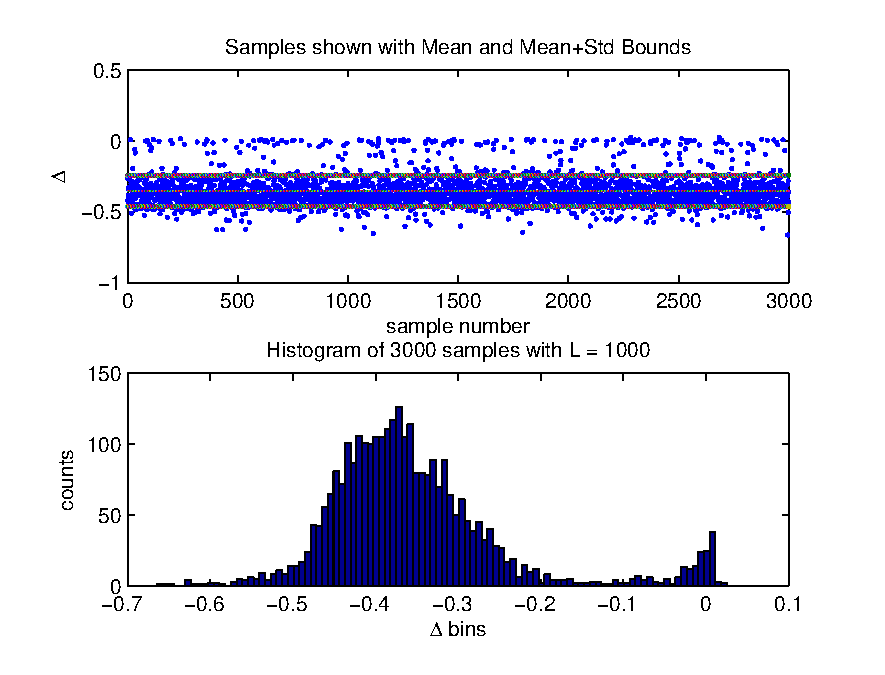
\includegraphics[scale=0.55]{TwoPopDynSampFig1.eps}
\caption{3000 samples with $\left(\mu_{rx},\mu_{ry},\sigma^2_{rx},\sigma^2_{ry},\mu_{x0},\mu_{y0},\sigma^2_{x0},\sigma^2_{y0}\right) = \left(3.8,3.5,0.05,0.05,0.4,0.2,0.1,0.1\right)$ and $\left(E,\tau\right)=\left(3,1\right)$ for $L=1000$ with ``zeroes removed''.}
\end{subfigure}
\begin{subfigure}[b]{0.4\textwidth}
\label{fig:TwoPopDynSampFig1_10000}
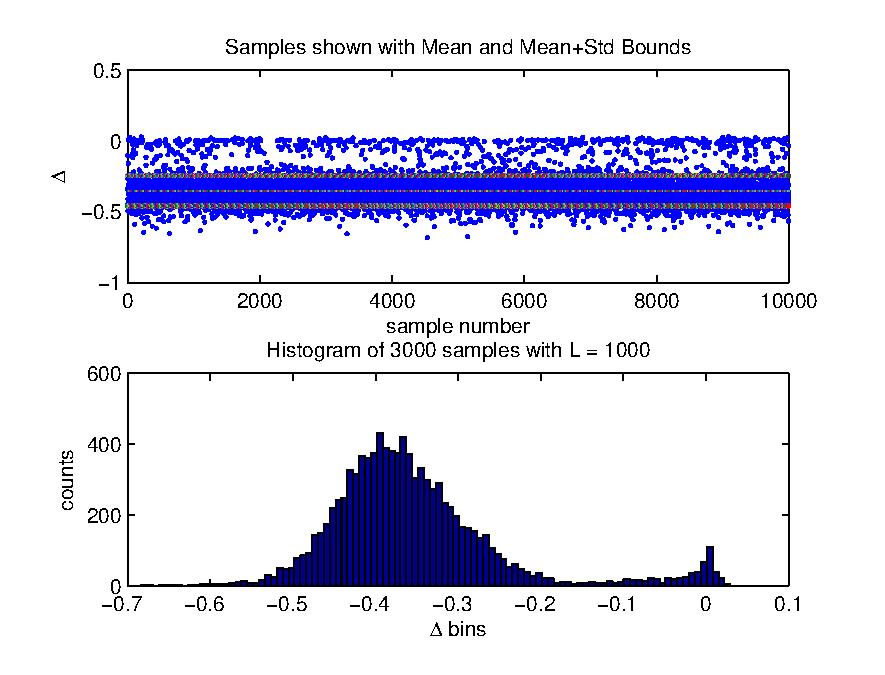
\includegraphics[scale=0.55]{TwoPopDynSampFig1_10000.eps}
\caption{10000 samples (ignore the histogram title) with $\left(\mu_{rx},\mu_{ry},\sigma^2_{rx},\sigma^2_{ry},\mu_{x0},\mu_{y0},\sigma^2_{x0},\sigma^2_{y0}\right) = \left(3.8,3.5,0.05,0.05,0.4,0.2,0.1,0.1\right)$ and $\left(E,\tau\right)=\left(3,1\right)$ for $L=1000$ with ``zeroes removed''.}
\end{subfigure}
\caption{}
\end{figure}

\begin{figure}[h!t]
\centering
\centering
\begin{subfigure}[b]{0.4\textwidth}
\label{fig:TwoPopDynSampFig2}
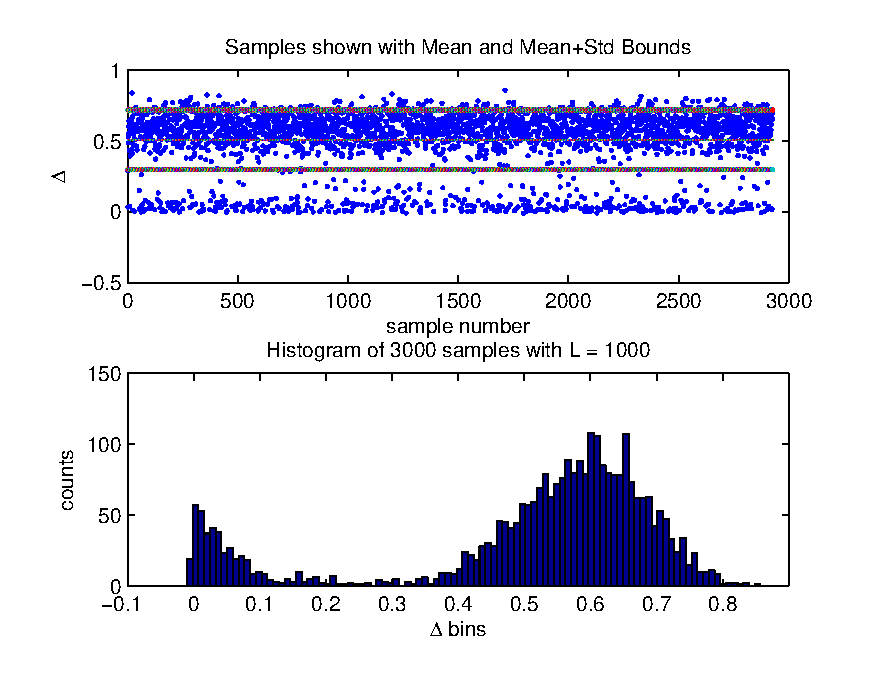
\includegraphics[scale=0.55]{TwoPopDynSampFig2.eps}
\caption{3000 samples with $\left(\mu_{rx},\mu_{ry},\sigma^2_{rx},\sigma^2_{ry},\mu_{x0},\mu_{y0},\sigma^2_{x0},\sigma^2_{y0}\right) = \left(3.1,3.9,0.05,0.05,0.4,0.2,0.1,0.1\right)$ and $\left(E,\tau\right)=\left(3,1\right)$ for $L=1000$ with ``zeroes removed'' and $(\beta_{xy},\beta_{yx})=(0.2,0.002)$.}
\end{subfigure}
\begin{subfigure}[b]{0.4\textwidth}
\label{fig:TwoPopDynSampFig3}
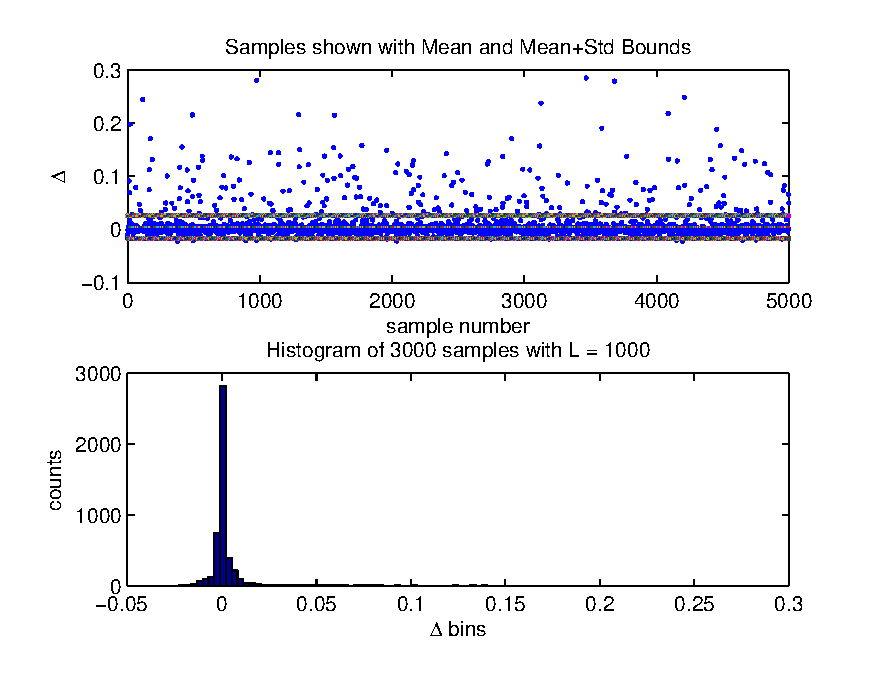
\includegraphics[scale=0.55]{TwoPopDynSampFig3.eps}
\caption{5000 samples (ignore the histogram title) with $\left(\mu_{rx},\mu_{ry},\sigma^2_{rx},\sigma^2_{ry},\mu_{x0},\mu_{y0},\sigma^2_{x0},\sigma^2_{y0}\right) = \left(3.5,3.5,0.05,0.05,0.4,0.4,0.1,0.1\right)$ and $\left(E,\tau\right)=\left(3,1\right)$ for $L=1000$ with ``zeroes removed'' and $(\beta_{xy},\beta_{yx})=(0.2,0.002)$.}
\end{subfigure}
\caption{}
\end{figure}

\section{Applying CCM to Known Dynamics}
The results shown above for the example presented by Sugihara appear to imply the following:
\begin{enumerate}
\item The CCM method is not robust with respect to the embedding dimension (i.e.\ $E$) or lag time step (i.e.\ $\tau$).
\item The CCM method can lead to results that agree with intuition for the presented example. 
\end{enumerate}
These points will be explored by applying the CCM to two very different sets of dynamics.  The first will explore a driven system by comparing the directed correlations calculated between the voltage and current time series of an RL circuit, and the second will explore the directed correlations found in the Lorenz system, which is known to be chaotic.

\subsection{RL Circuit}
An RL circuit is described as
$$
\dot{I} = \frac{V}{L} - \frac{R}{L} I\;\;,
$$
where $I$ is the current, $V$ is the voltage, $R$ is the resistance, and $L$ is the inductance.  The driving time series will be the voltage $V$ and the response times series will be the current $I$.  The resistance and inductance will be considered fixed.

Consider an RL circuit with $(R,L) = (0.5,10)$.  If the voltage times series $V$ consists of two triangular pulses separated by constant spans of $V=0$, then the current times series $I$ will likewise has two maximums as seen in Figure \ref{fig:RL_trigsignals}.  The directed correlations $C_{VI}$ and $C_{IV}$ can be plotted as a function of the embedding dimension $E$ to show that $C_{VI}>C_{IV}$ for $E=2,3,\ldots,10$.  This plot is Figure \ref{fig:RL_trigsignalsCCM}.
\begin{figure}[h!t]
\centering
\begin{subfigure}[b]{0.4\textwidth}
\label{fig:RL_trigsignals}
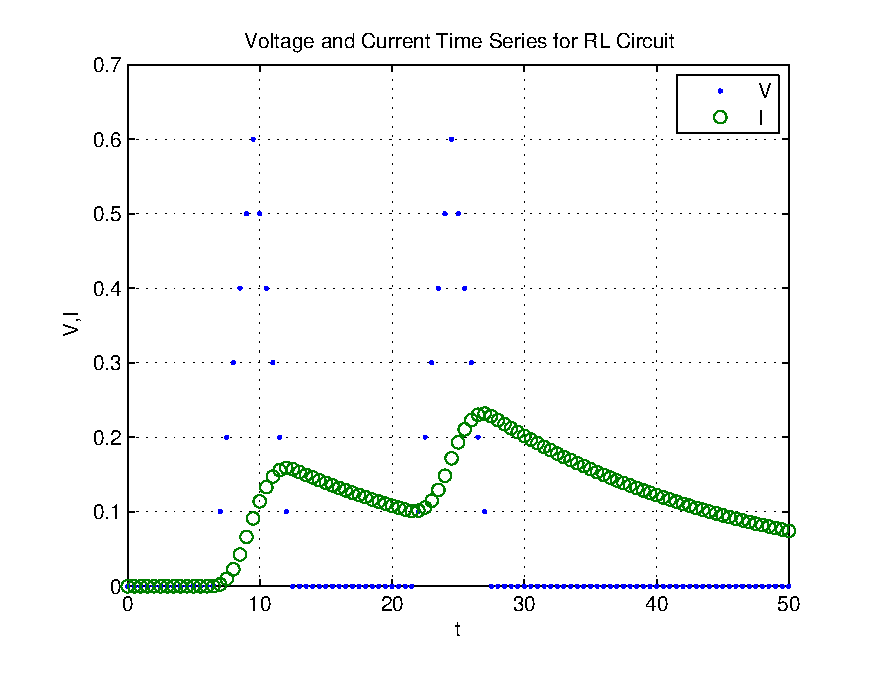
\includegraphics[scale=0.55]{RL_trigsignals.eps}
\caption{$(R,L) = (0.5,10)$}
\end{subfigure}
\begin{subfigure}[b]{0.4\textwidth}
\label{fig:RL_trigsignalsCCM}
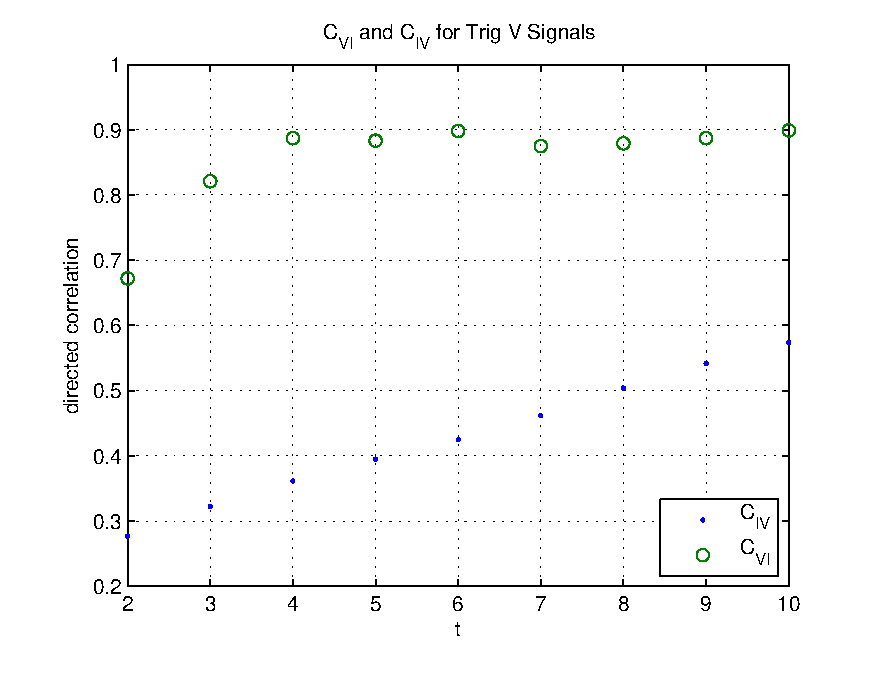
\includegraphics[scale=0.55]{RL_trigsignalsCCM.eps}
\caption{$(R,L) = (0.5,10)$ with $\left(E,L,\tau\right)=\left(2,100,1\right)$}
\end{subfigure}
\caption{}
\end{figure}
This result (i.e.\ that the system is directionally correlated from $V$ to $I$) is expected because $V\Rightarrow I$ (i.e.\ the voltage drives the current).

Consider the case when $V$ is a discrete sine function; see Figure \ref{fig:RL_sinsignals} for a plot of the $V$ and $I$ times series.  The values of $C_{VI}$ and $C_{IV}$ are different than they were in the example of the previous paragraph but the general relationship is the same, i.e.\ $C_{VI}>C_{IV}$ for $E=2,3,\ldots,10$.  See Figure \ref{fig:RL_sinsignalsCCM}.
\begin{figure}[h!t]
\centering
\begin{subfigure}[b]{0.4\textwidth}
\label{fig:RL_sinsignals}
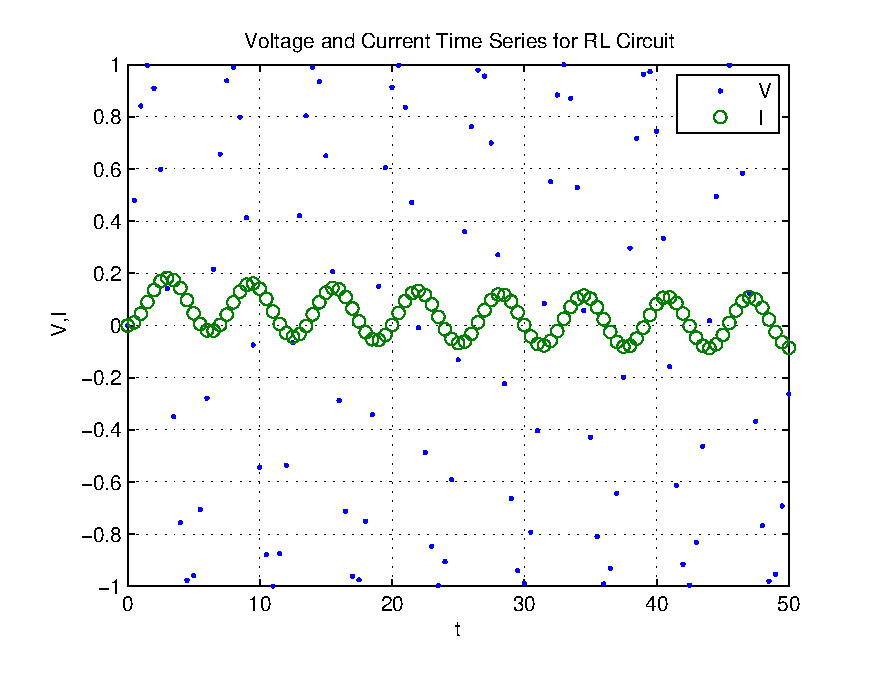
\includegraphics[scale=0.55]{RL_sinsignals.eps}
\caption{$(R,L) = (0.5,10)$}
\end{subfigure}
\begin{subfigure}[b]{0.4\textwidth}
\label{fig:RL_sinsignalsCCM}
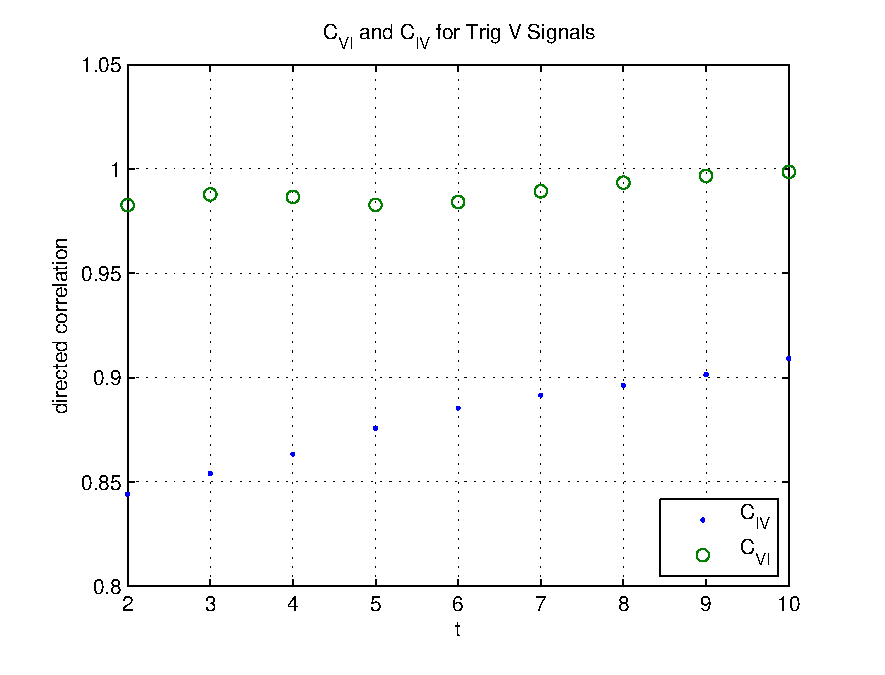
\includegraphics[scale=0.55]{RL_sinsignalsCCM.eps}
\caption{$(R,L) = (0.5,10)$ with $\left(E,L,\tau\right)=\left(2,100,1\right)$}
\end{subfigure}
\caption{}
\end{figure}

The ``non-robust'' features of the directed correlations (with respect to $E$) can be recovered for the RL circuit by setting each point of $V$ to be a random value.  While such a voltage time series may be suspect (i.e.\ it results in possibly non-stationary current response time series), it will illustrate the same $E$-dependent behaviour of the directed correlations that was seen with the Sugihara example.  Consider the $V$ and $I$ times series of Figure \ref{fig:RL_randsignals}, where $V$ is a set of pseudo-random numbers generated with Matlab.  The plot of $C_{VI}$ and $C_{IV}$ for $E=2,3,\ldots,10$ (see Figure \ref{fig:RL_randsignalsCCM}) shows that $C_{VI}>C_{IV}$ if $E\ge 4$ but $C_{VI}<C_{IV}$ if $E<4$.
\begin{figure}[h!t]
\centering
\begin{subfigure}[b]{0.4\textwidth}
\label{fig:RL_randsignals.eps}
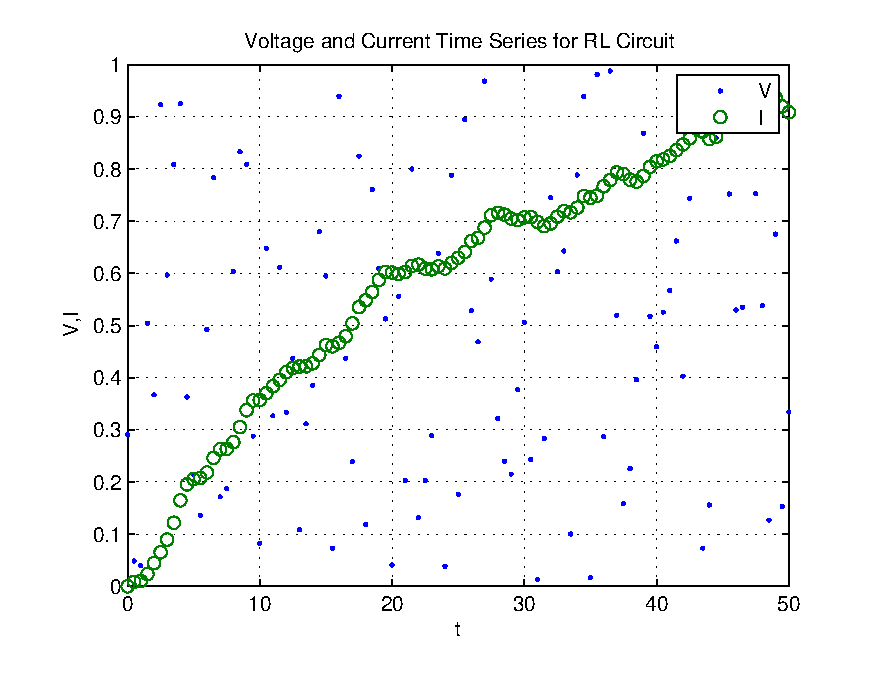
\includegraphics[scale=0.55]{RL_randsignals.eps}
\caption{$(R,L) = (0.5,10)$}
\end{subfigure}
\begin{subfigure}[b]{0.4\textwidth}
\label{fig:RL_randsignalsCCM}
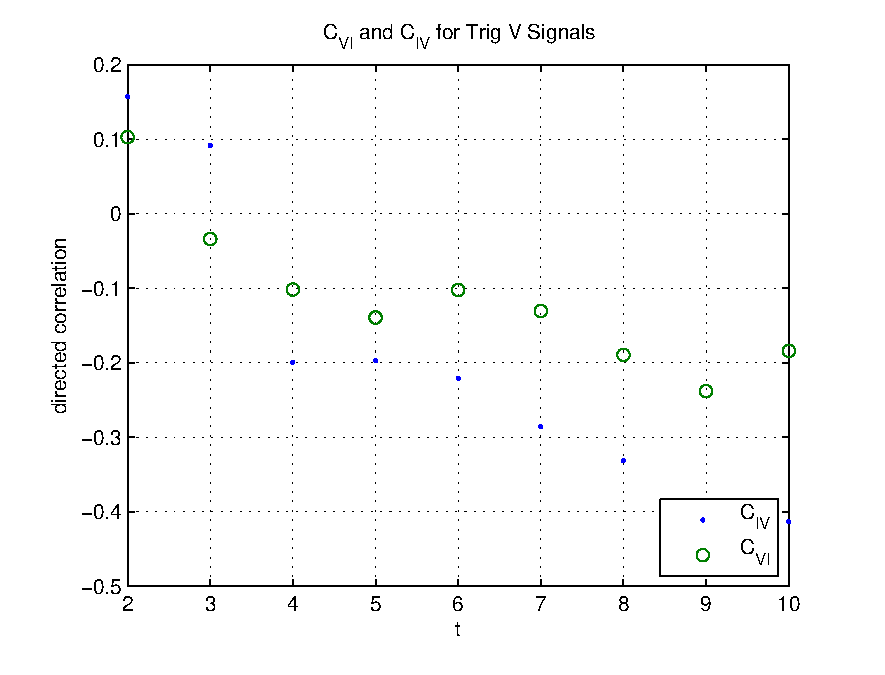
\includegraphics[scale=0.55]{RL_randsignalsCCM.eps}
\caption{$(R,L) = (0.5,10)$ with $\left(E,L,\tau\right)=\left(2,100,1\right)$}
\end{subfigure}
\caption{}
\end{figure}
 
These results seem to imply that the robustness of the CCM method may be related to the autocorrelation of the ``driving'' time series.  This idea will be explored after the next section.

\subsection{Lorenz System}
Consider the following system of equations:
\begin{eqnarray*}
\dot{x} &=& \sigma\left(y-x\right)\\
\dot{y} &=& \rho x-y-xz\\
\dot{z} &=& xy - \beta z
\end{eqnarray*}
If $(\sigma,\beta,\rho)=(10,8/3,28)$, then the system's directed correlations are as follows:
\begin{eqnarray*}
C_{xy} &\approx & 0.91\\
C_{yx} &\approx & 0.94\\
C_{xz} &\approx & 0.11\\
C_{zx} &\approx & 0.88\\
C_{yz} &\approx & 0.08\\
C_{zy} &\approx & 0.45
\end{eqnarray*}
where $x(t)$, $y(t)$, and $z(t)$ are defined by the dynamical system at the beginning of this section.  These results seem to imply $z\Rightarrow x$ and $z\Rightarrow y$ with no conclusion for the relationship between $x$ and $y$.  These results seem confusing.  In particular, it seems to make sense that $z$ could be a stronger driver of $y$ than $y$ is of $z$ (i.e.\ $z\Rightarrow y$) but the implication that $z$ is a stronger driver of $x$ than $x$ is of $z$ (i.e.\ $z\Rightarrow x$) is more difficult to interpret given that $z$ only affects $x$ through $y$.

If $(\sigma,\beta,\rho)=(0.01,8/3,28)$, then the system's directed correlations are as follows:
\begin{eqnarray*}
C_{xy} &\approx & 0.79\\
C_{yx} &\approx & -0.12\\
C_{xz} &\approx & 0.90\\
C_{zx} &\approx & -0.74\\
C_{yz} &\approx & 0.47\\
C_{zy} &\approx & 0.71
\end{eqnarray*}
which implies $x\Rightarrow y$, $z\Rightarrow y$, and $x\Rightarrow z$.  Both $x\Rightarrow y$ and $x\Rightarrow z$ seems to make intuitive sense given the smaller $\sigma$ in this example versus the previous example, and $z\Rightarrow y$ is consistent with the previous example which, again, makes sense because neither $\rho$ nor $\beta$ was changed.

If $(\sigma,\beta,\rho)=(10,0.01,28)$, then the system's directed correlations are as follows:
\begin{eqnarray*}
C_{xy} &\approx & -1\\
C_{yx} &\approx & 1\\
C_{xz} &\approx & 0.02\\
C_{zx} &\approx & 0.30\\
C_{yz} &\approx & 0.01\\
C_{zy} &\approx & 0.40
\end{eqnarray*}

This section will be expanded $\ldots$

\end{document}
